\documentclass [11pt, letterpaper] {article}
\input {headings}
\newcommand \recipeName {Roasted Sweet Potatoes with Paprika}
\newcommand \fileName {SweetPotatoPaprika}
\chead {\recipeName}

\begin {document}
\input {title}


The Boniato sweet potato (also known as Camote sweet potato or as white sweet potato) has a purple skin and firm white flesh. When you peel them, they will immediately turn dark. To prevent this you need to use acid --- I chose lemon. The combination of the natural sweetness of these potatoes with the paprika is great. I prepared this dish and and the next day I was having it with a bit of salad that had some sherry vinegar, the combination of the spicy sweet potatoes with the vinegar was very pleasant. Thus I added the vinegar to the recipe. 


\begin{description}

\item[Ingredients:]\ \\
	\begin{itemize}
	\item 2 2/1 to 3 pounds of Boniato Sweet Potatoes
	\item Two lemons
	\item 1 teaspoon of salt
	\item 2 Tablespoons of paprika
	\item 2 Tablespoons of olive oil
	\item 1 teaspoon of sherry vinegar
	\end{itemize}

\item[Equipment:]\ \\
	\begin{itemize}
	\item rimmed light-coloured baking sheet
	\item large bowl
	\item aluminum foil
        \item cooking spray
	\end{itemize}
\item[Procedure:]\ \\

	\begin{enumerate}
	\item {\bf Peel and dice potatoes}
	\begin{itemize}
	\item Cut up one lemon and leave nearby.
        \item Peel each potato removing all small indentations and any dark green spot under the peel. 
	\item Immediately rub the lemon half on the freshly peeled potato.
        \item Cut potatoes into one-inch cubes.
        \item Immediately squeeze the second lemon on top of the cubes and toss them well into the lemon juice. 
        \item Let it sit for a few minutes and then drain the lemon juice from the bowl.
        \item Sprinkle the diced potatoes with salt, mix well and let it sit for at least 30 minutes.
	\end{itemize}
	
	\item {\bf Season and roast potatoes }
	\begin{itemize}
	\item Turn oven to 325F and place an empty light-coloured rimmed baking sheet in the oven.
	\item Drain any water that accumulated at the bottom of the bowl from the salted diced potatoes.
	\item Sprinkle potatoes with paprika, stirring with a rubber spatula.
	\item Drizzle the olive oil over the potatoes and stir well.
        \item Remove the hot baking sheet from the oven and dump the potatoes into it, scrapping the oil from the bowl with the spatula.
        \item Spray the shiny side of a piece of aluminum foil that is large enough to completely cover the baking sheet.
        \item Completely cover the baking sheet with the foil with the shiny side down, closing the edges well so that the potatoes will steam.
        \item Roast covered for about one hour until the potatoes are tender when pierced with a sharp knife.
        \item Turn the oven temperature to 400F.
        \item Remove the foil, shake the pan or use a rubber spatula to loosen any potato piece that may be stuck to the pan.
        \item Return the uncovered potatoes to the oven and roast for another 20 minutes or so until the potatoes look roasted but are not too dry.
        \item Remove from oven and sprinkle the vinegar on top. Taste and add more vinegar if desired.
	\end{itemize}

	\end{enumerate}
\end{description}
\begin{table}
\begin{tabular}{cccc}
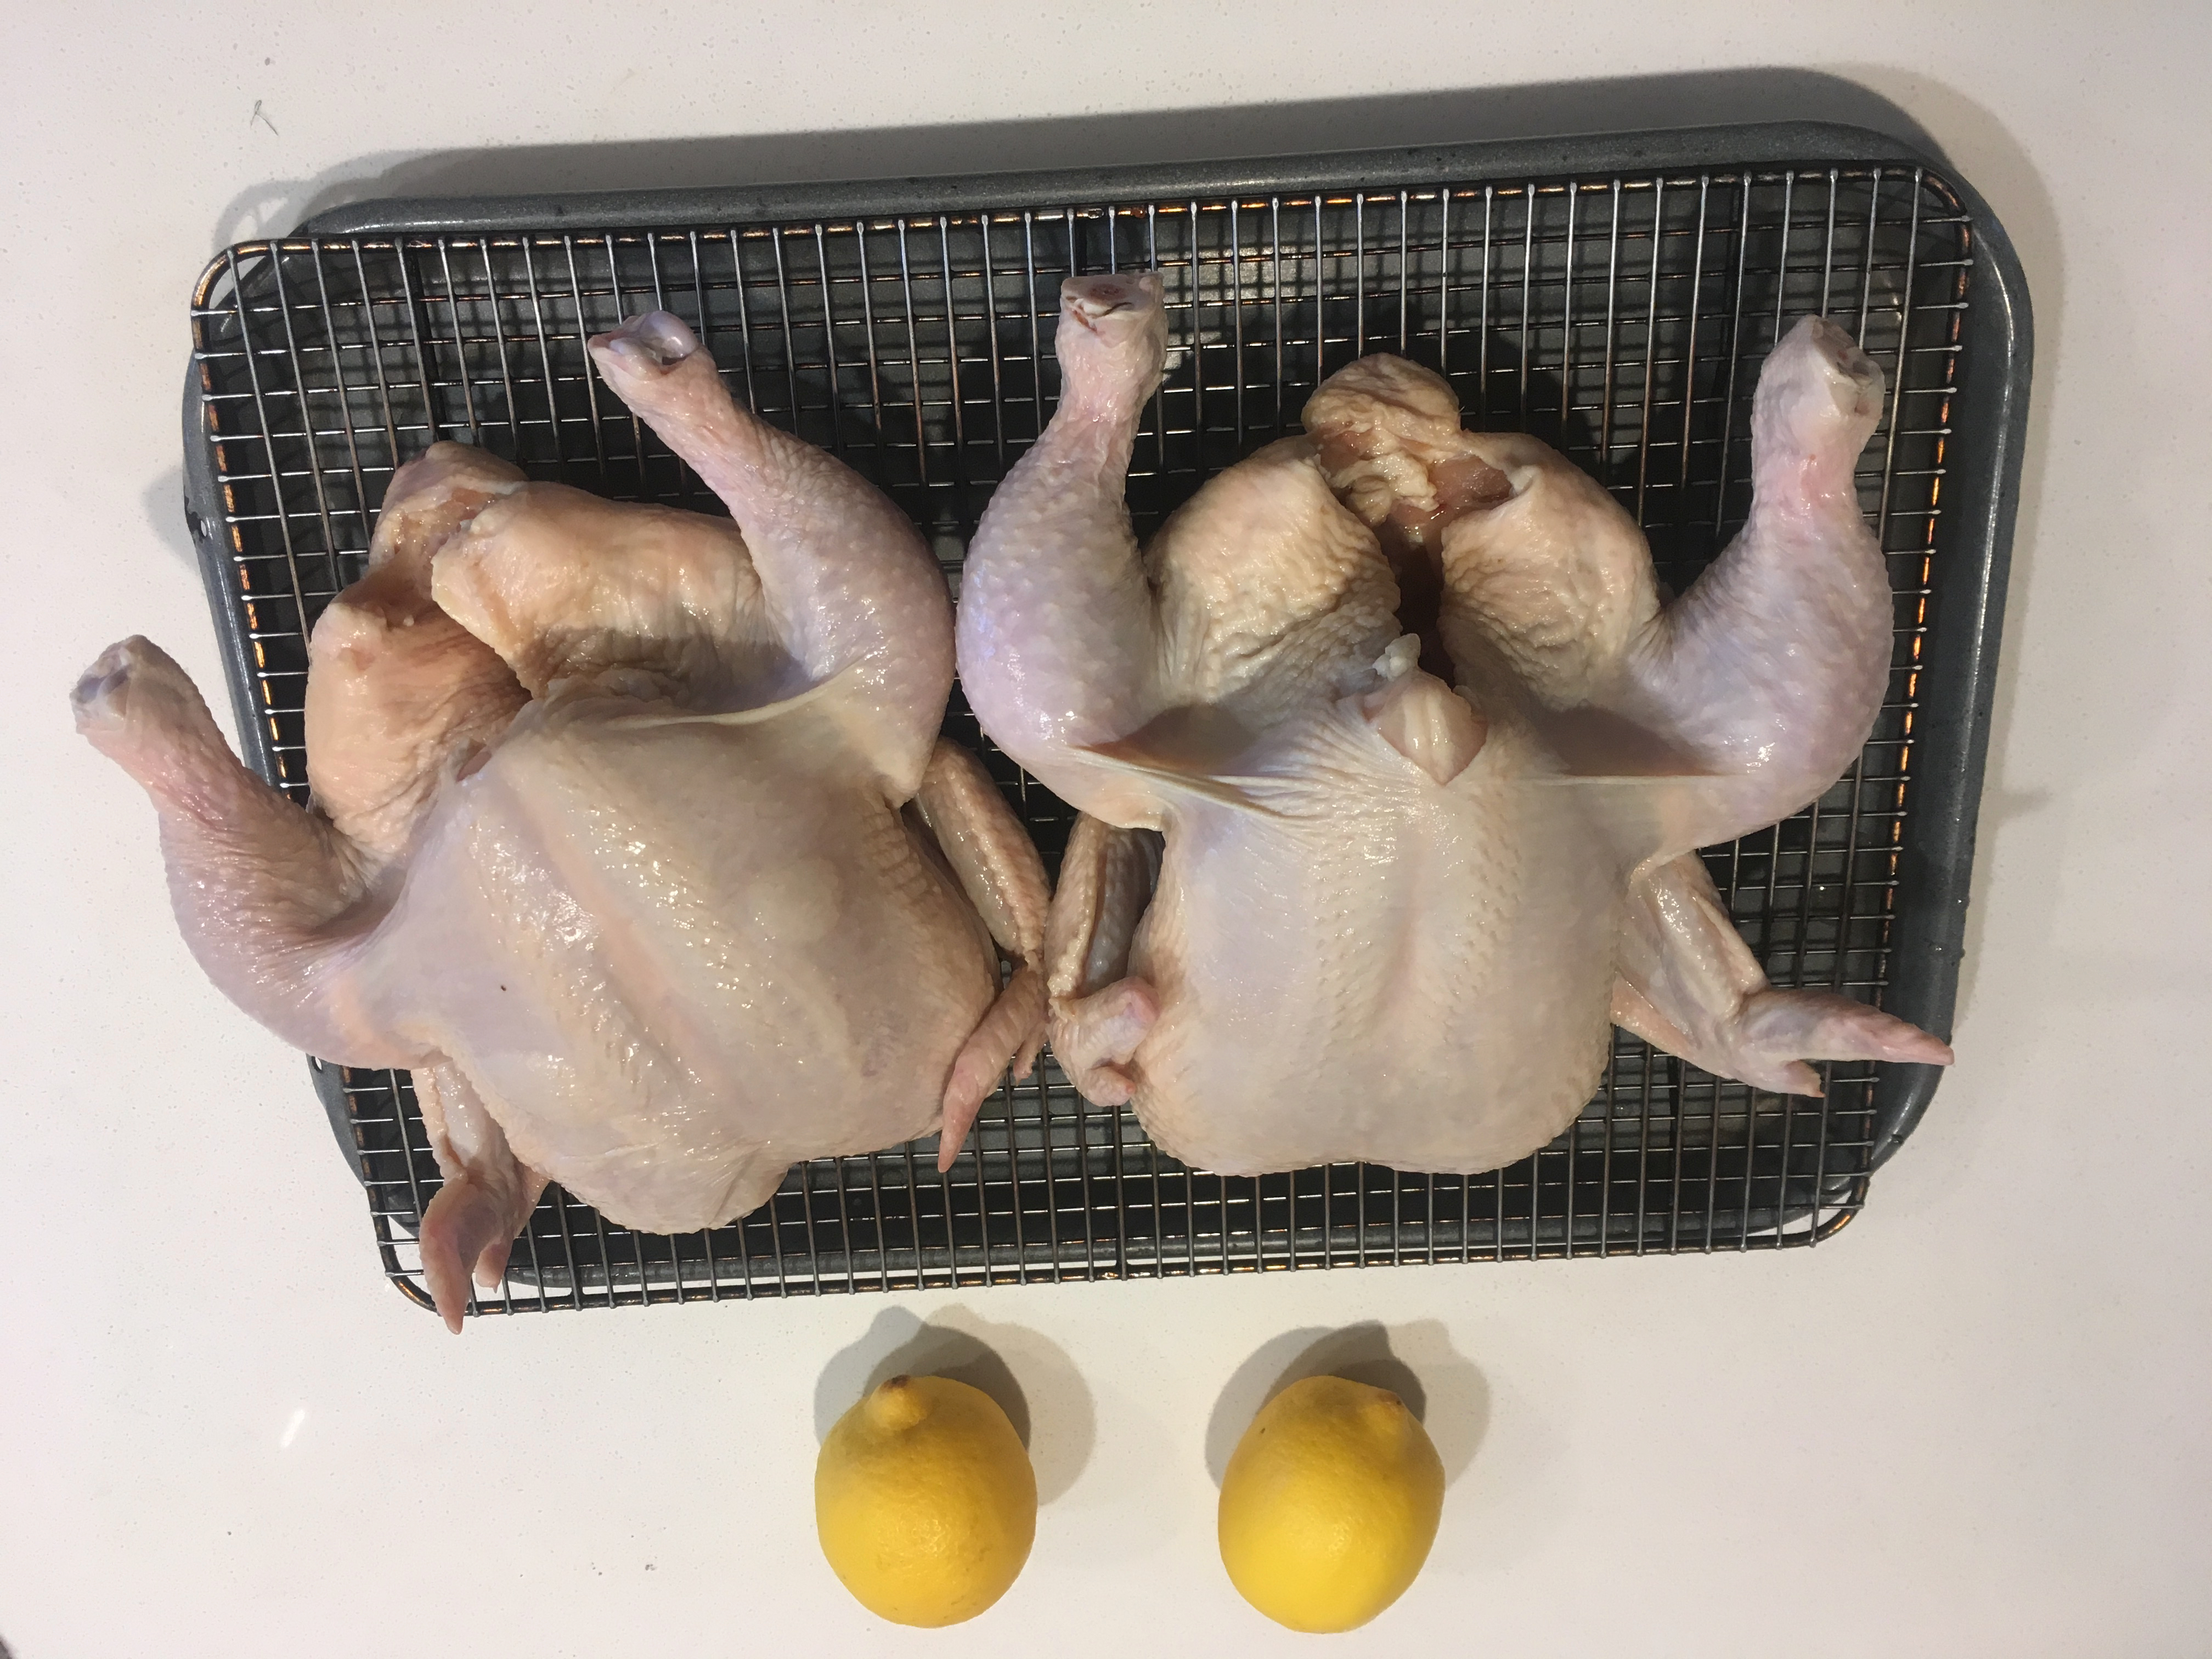
\includegraphics[width=0.25\textwidth]{\imageDir/\fileName/IMG_3197.jpg} &
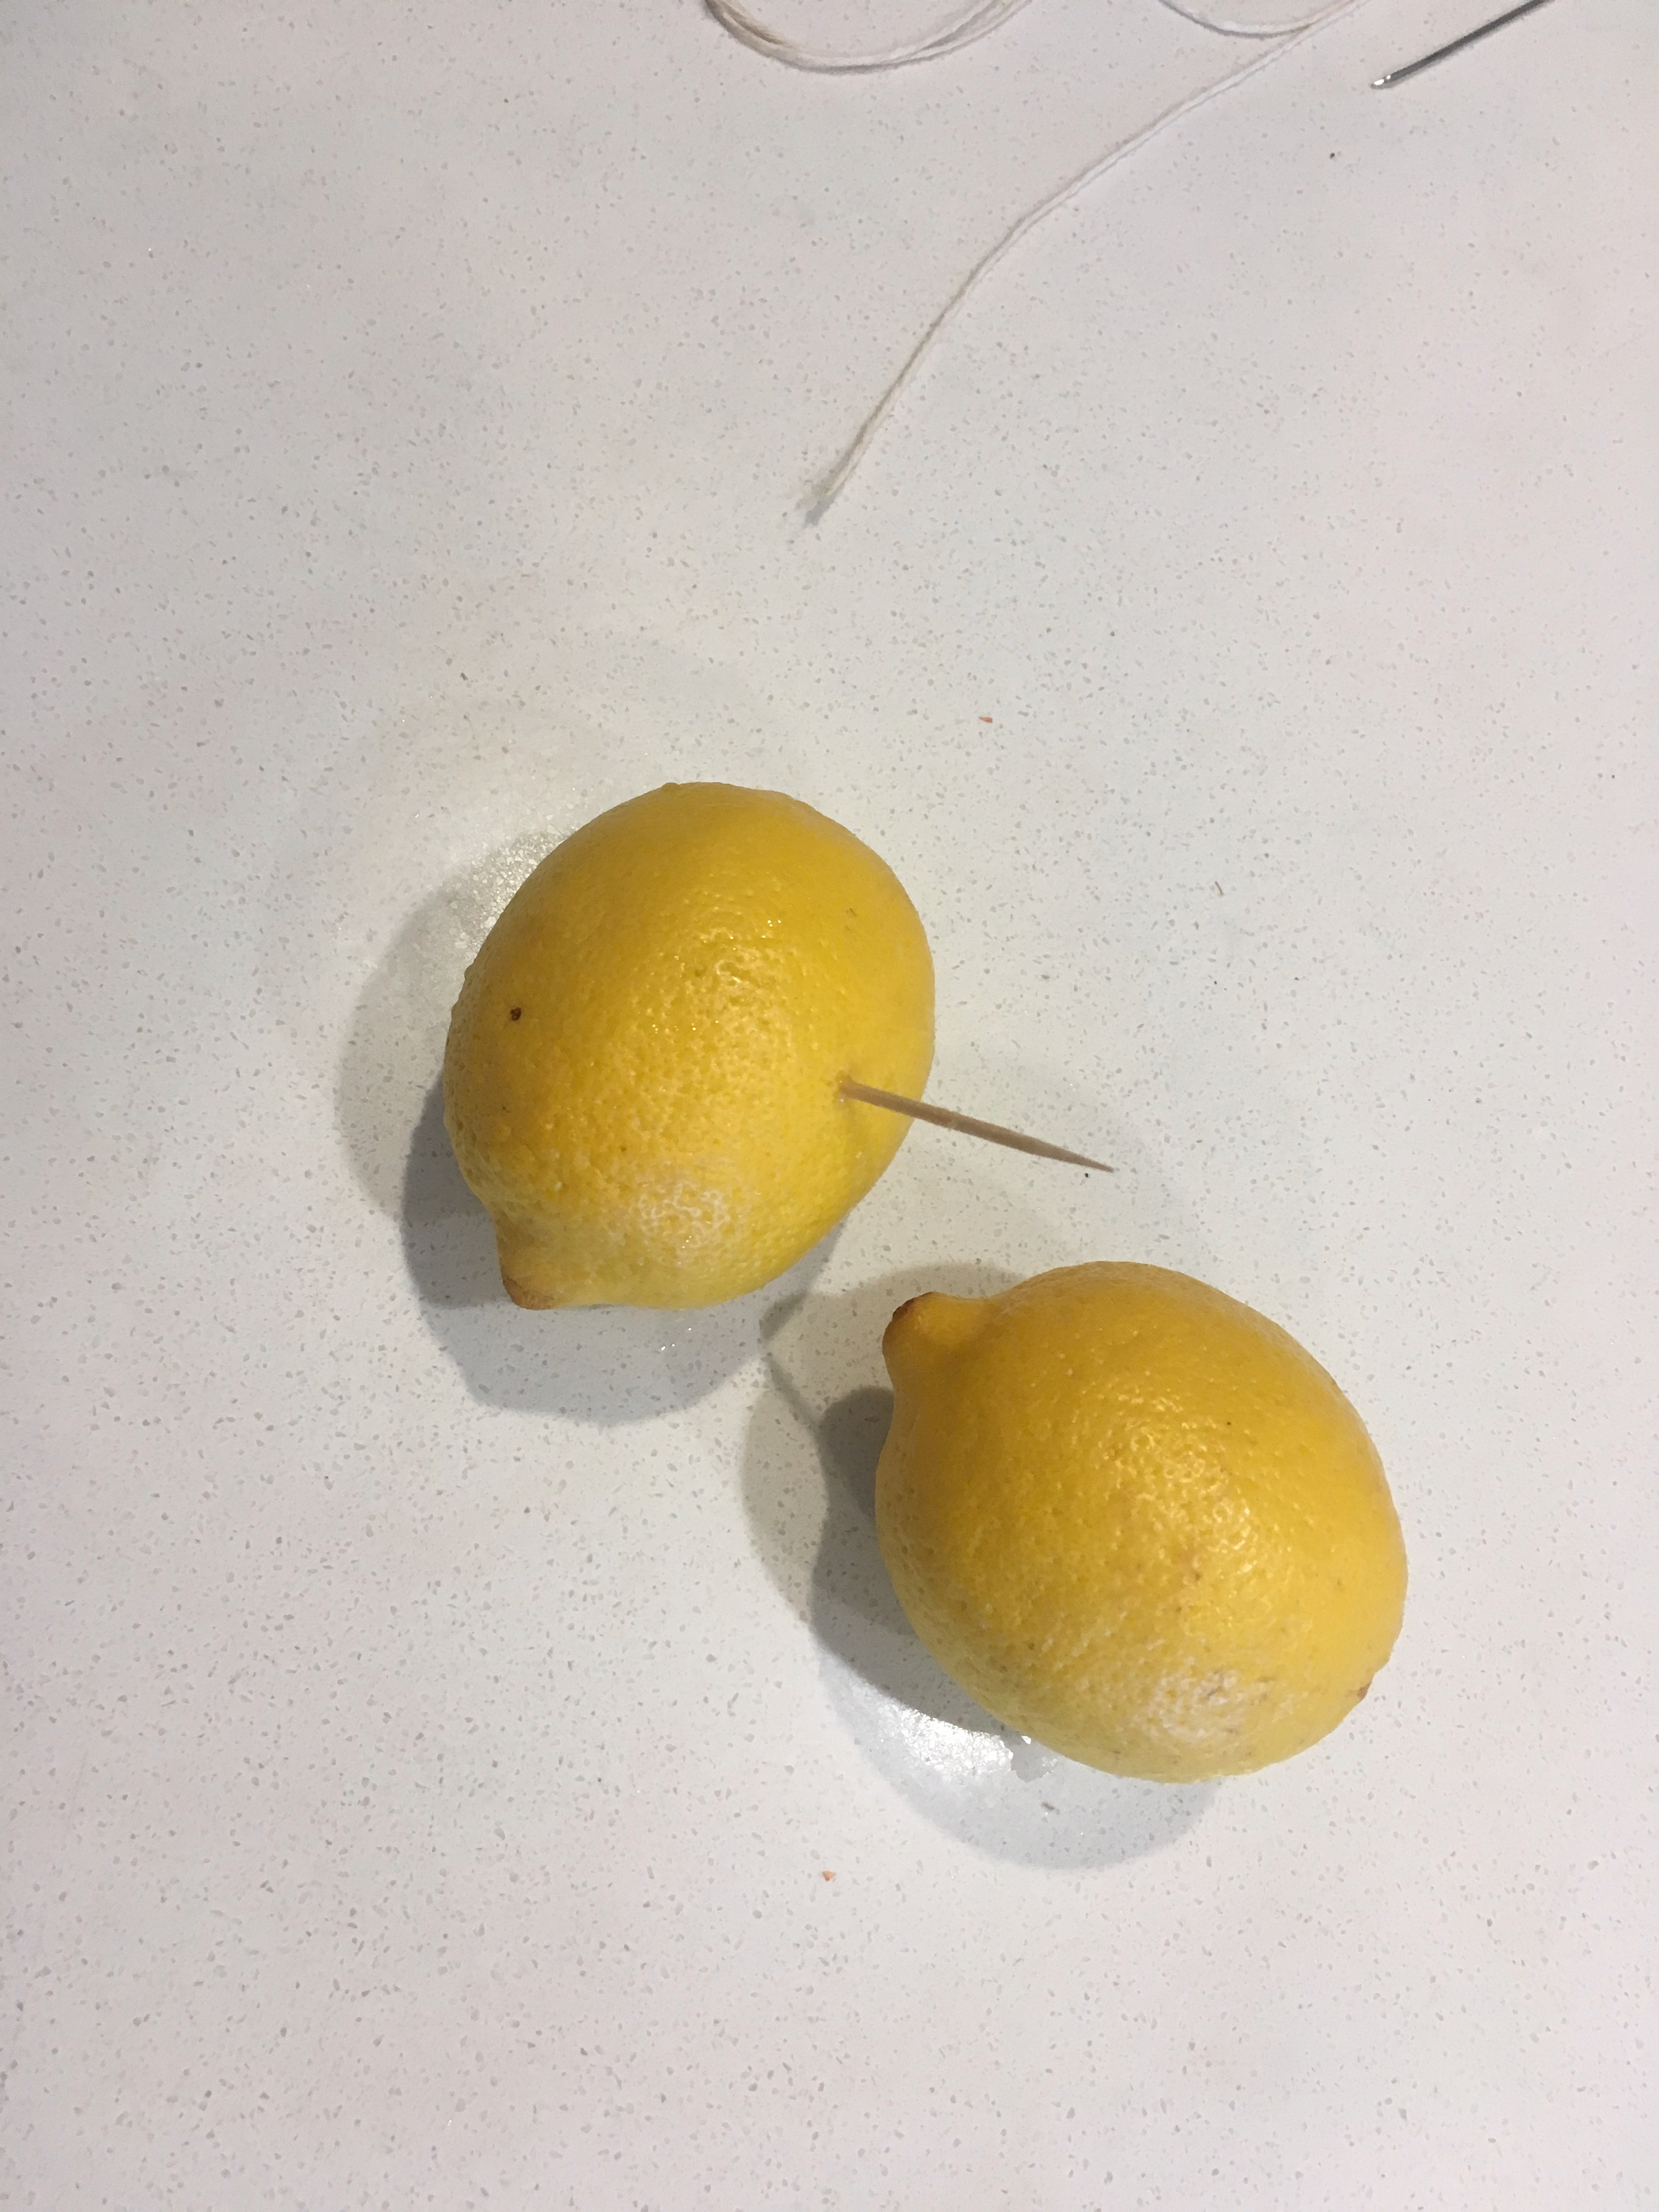
\includegraphics[width=0.25\textwidth]{\imageDir/\fileName/IMG_3212.jpg} &
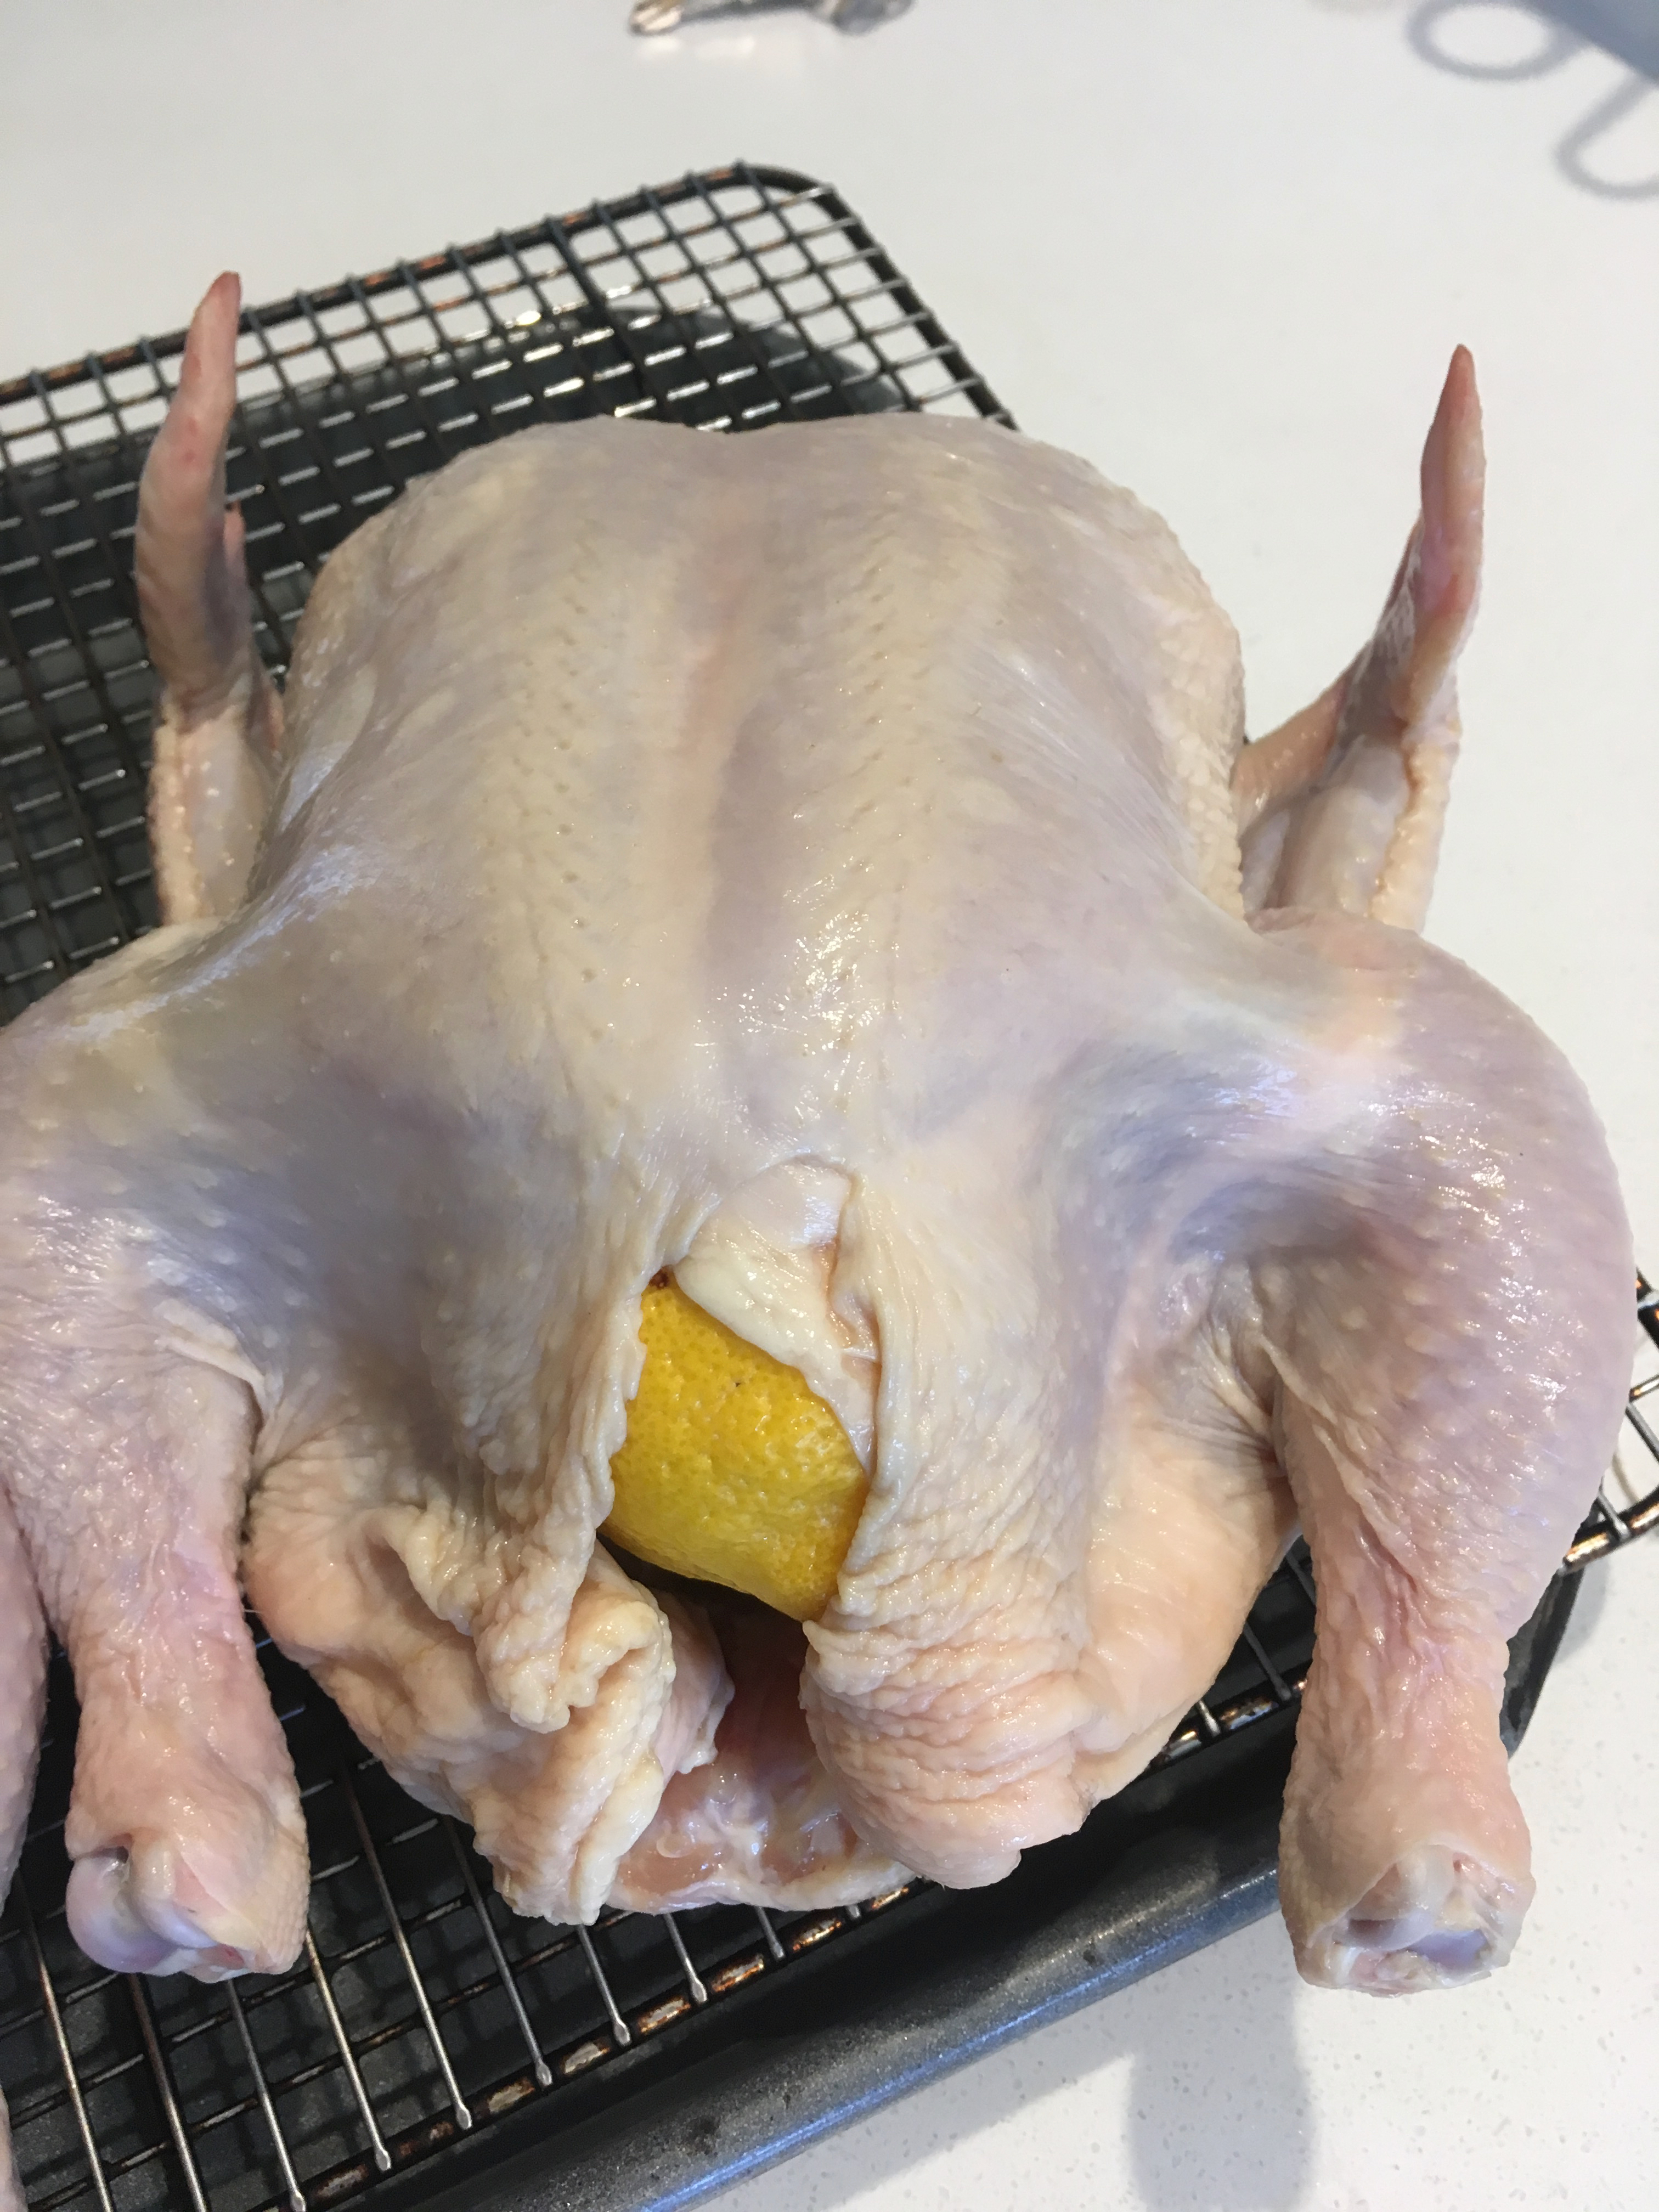
\includegraphics[width=0.25\textwidth]{\imageDir/\fileName/IMG_3213.jpg} \\
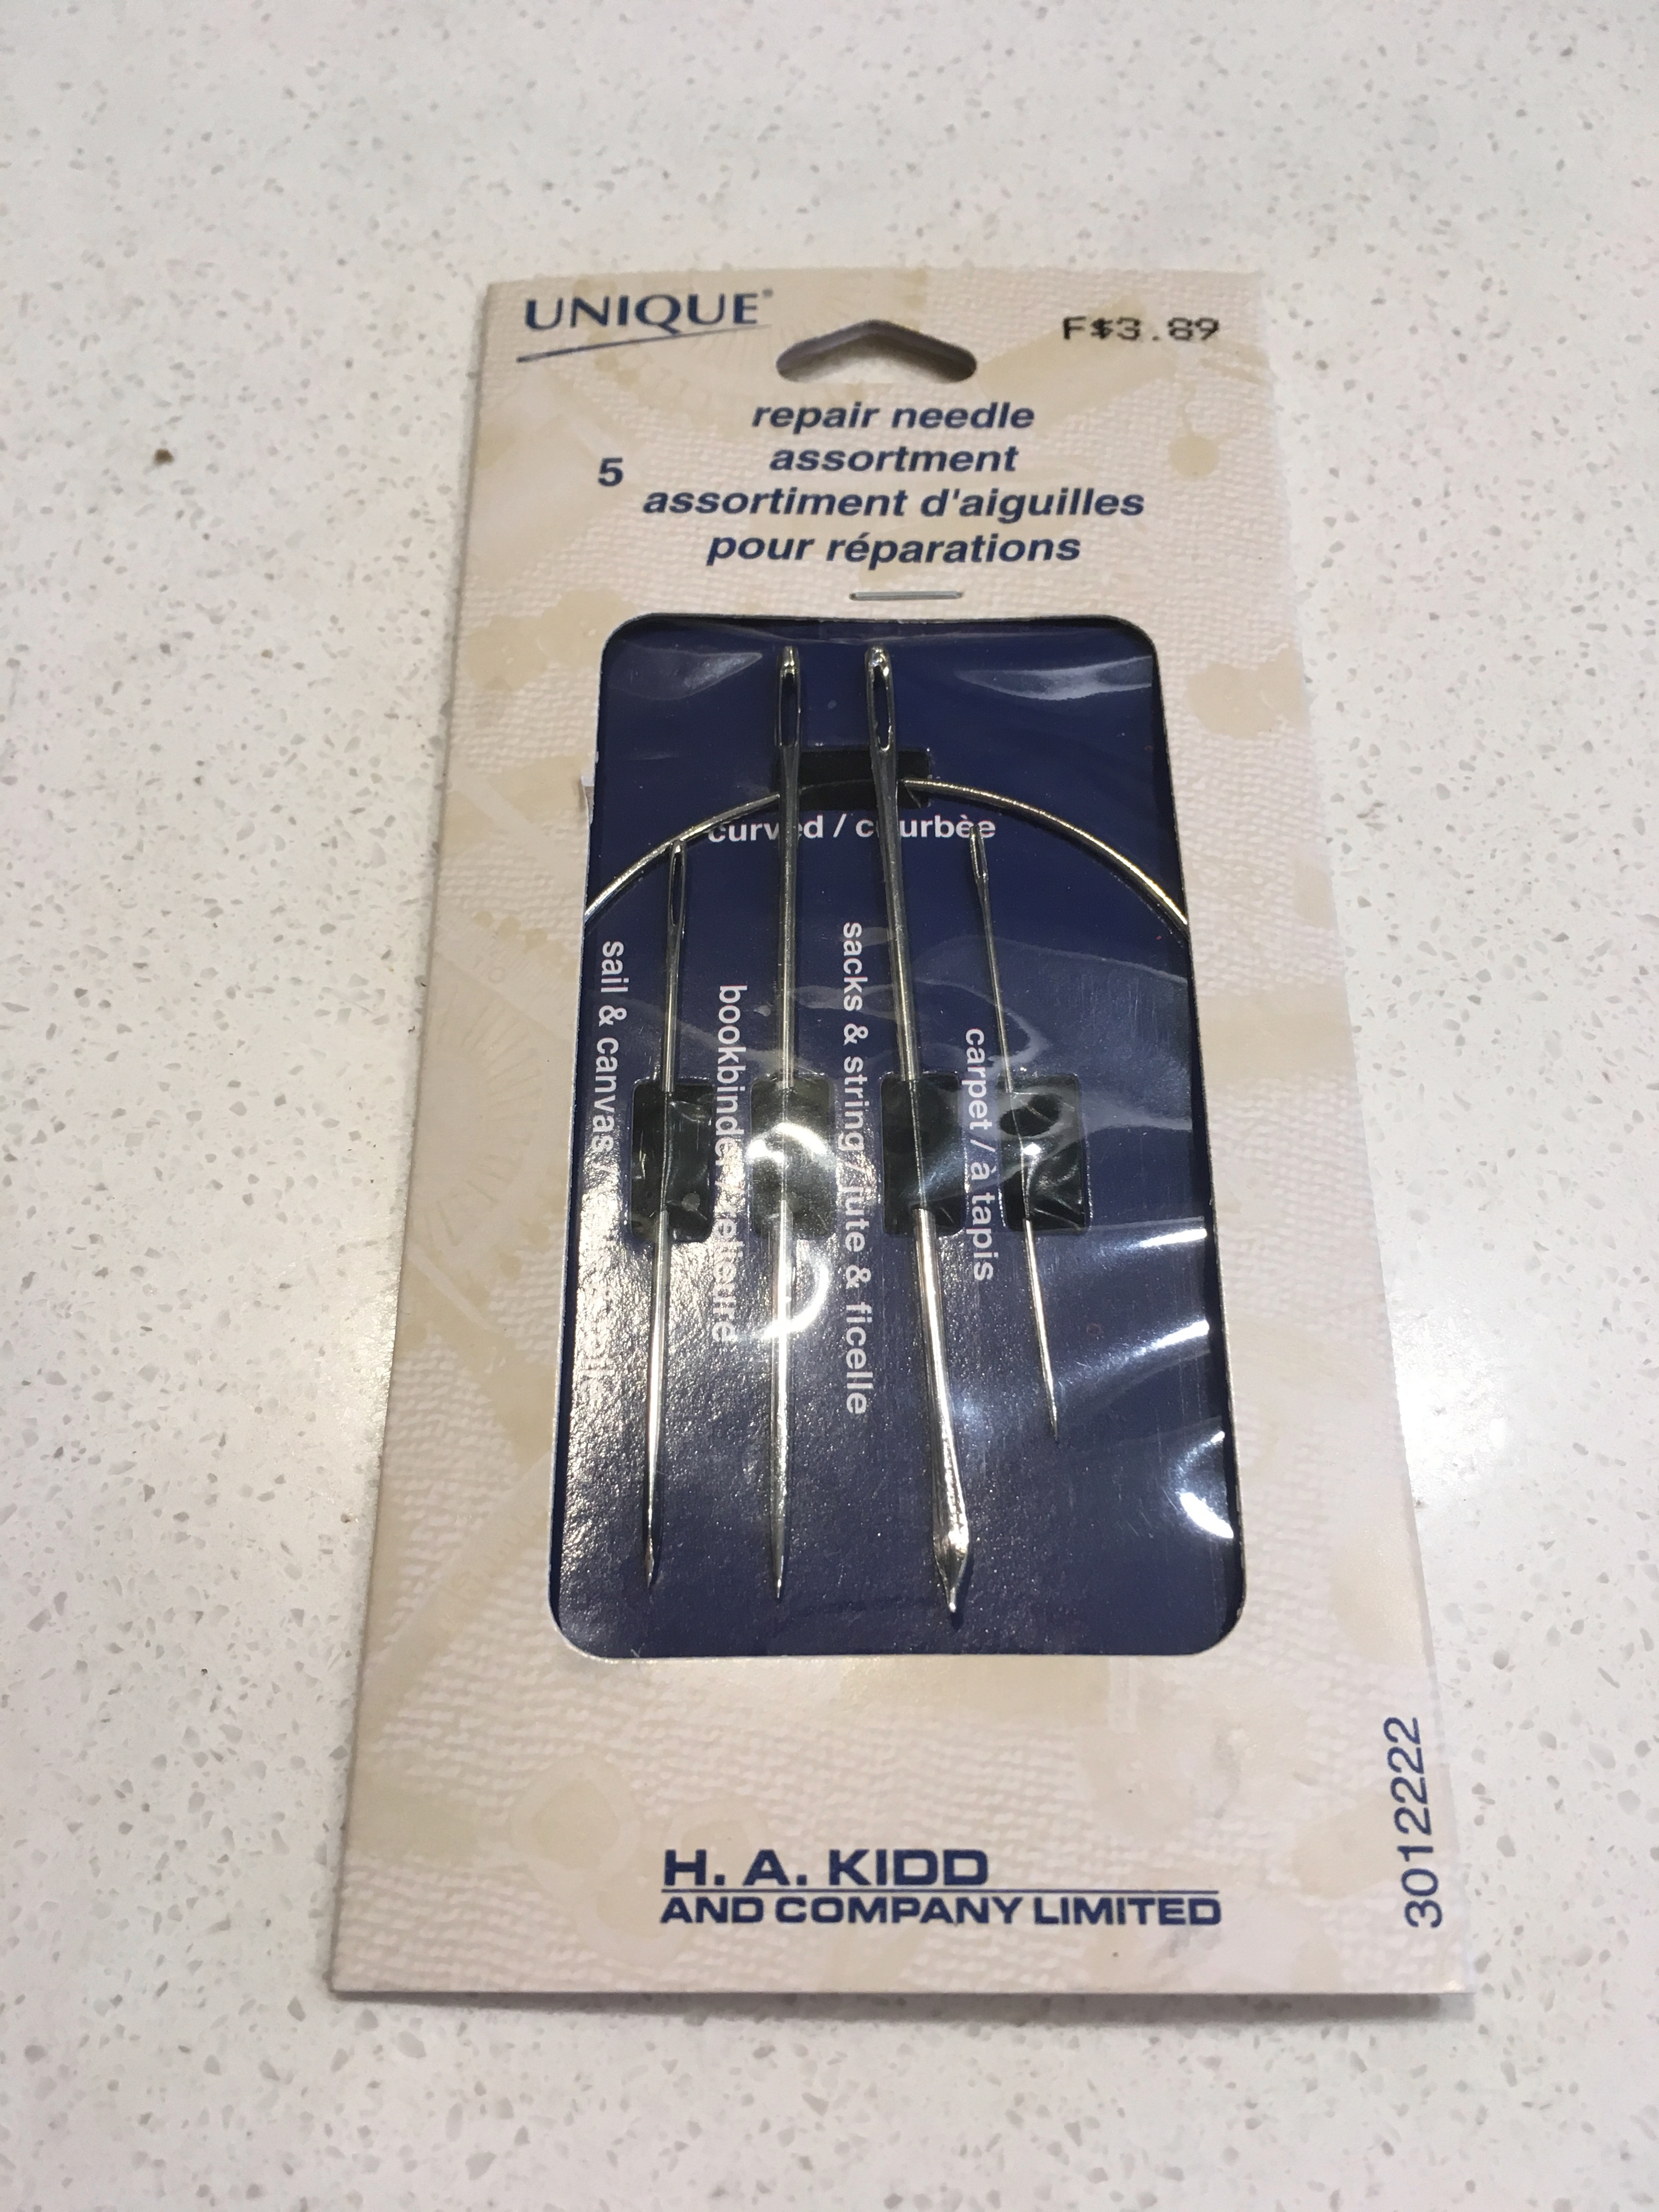
\includegraphics[width=0.25\textwidth]{\imageDir/\fileName/IMG_3206.jpg} &
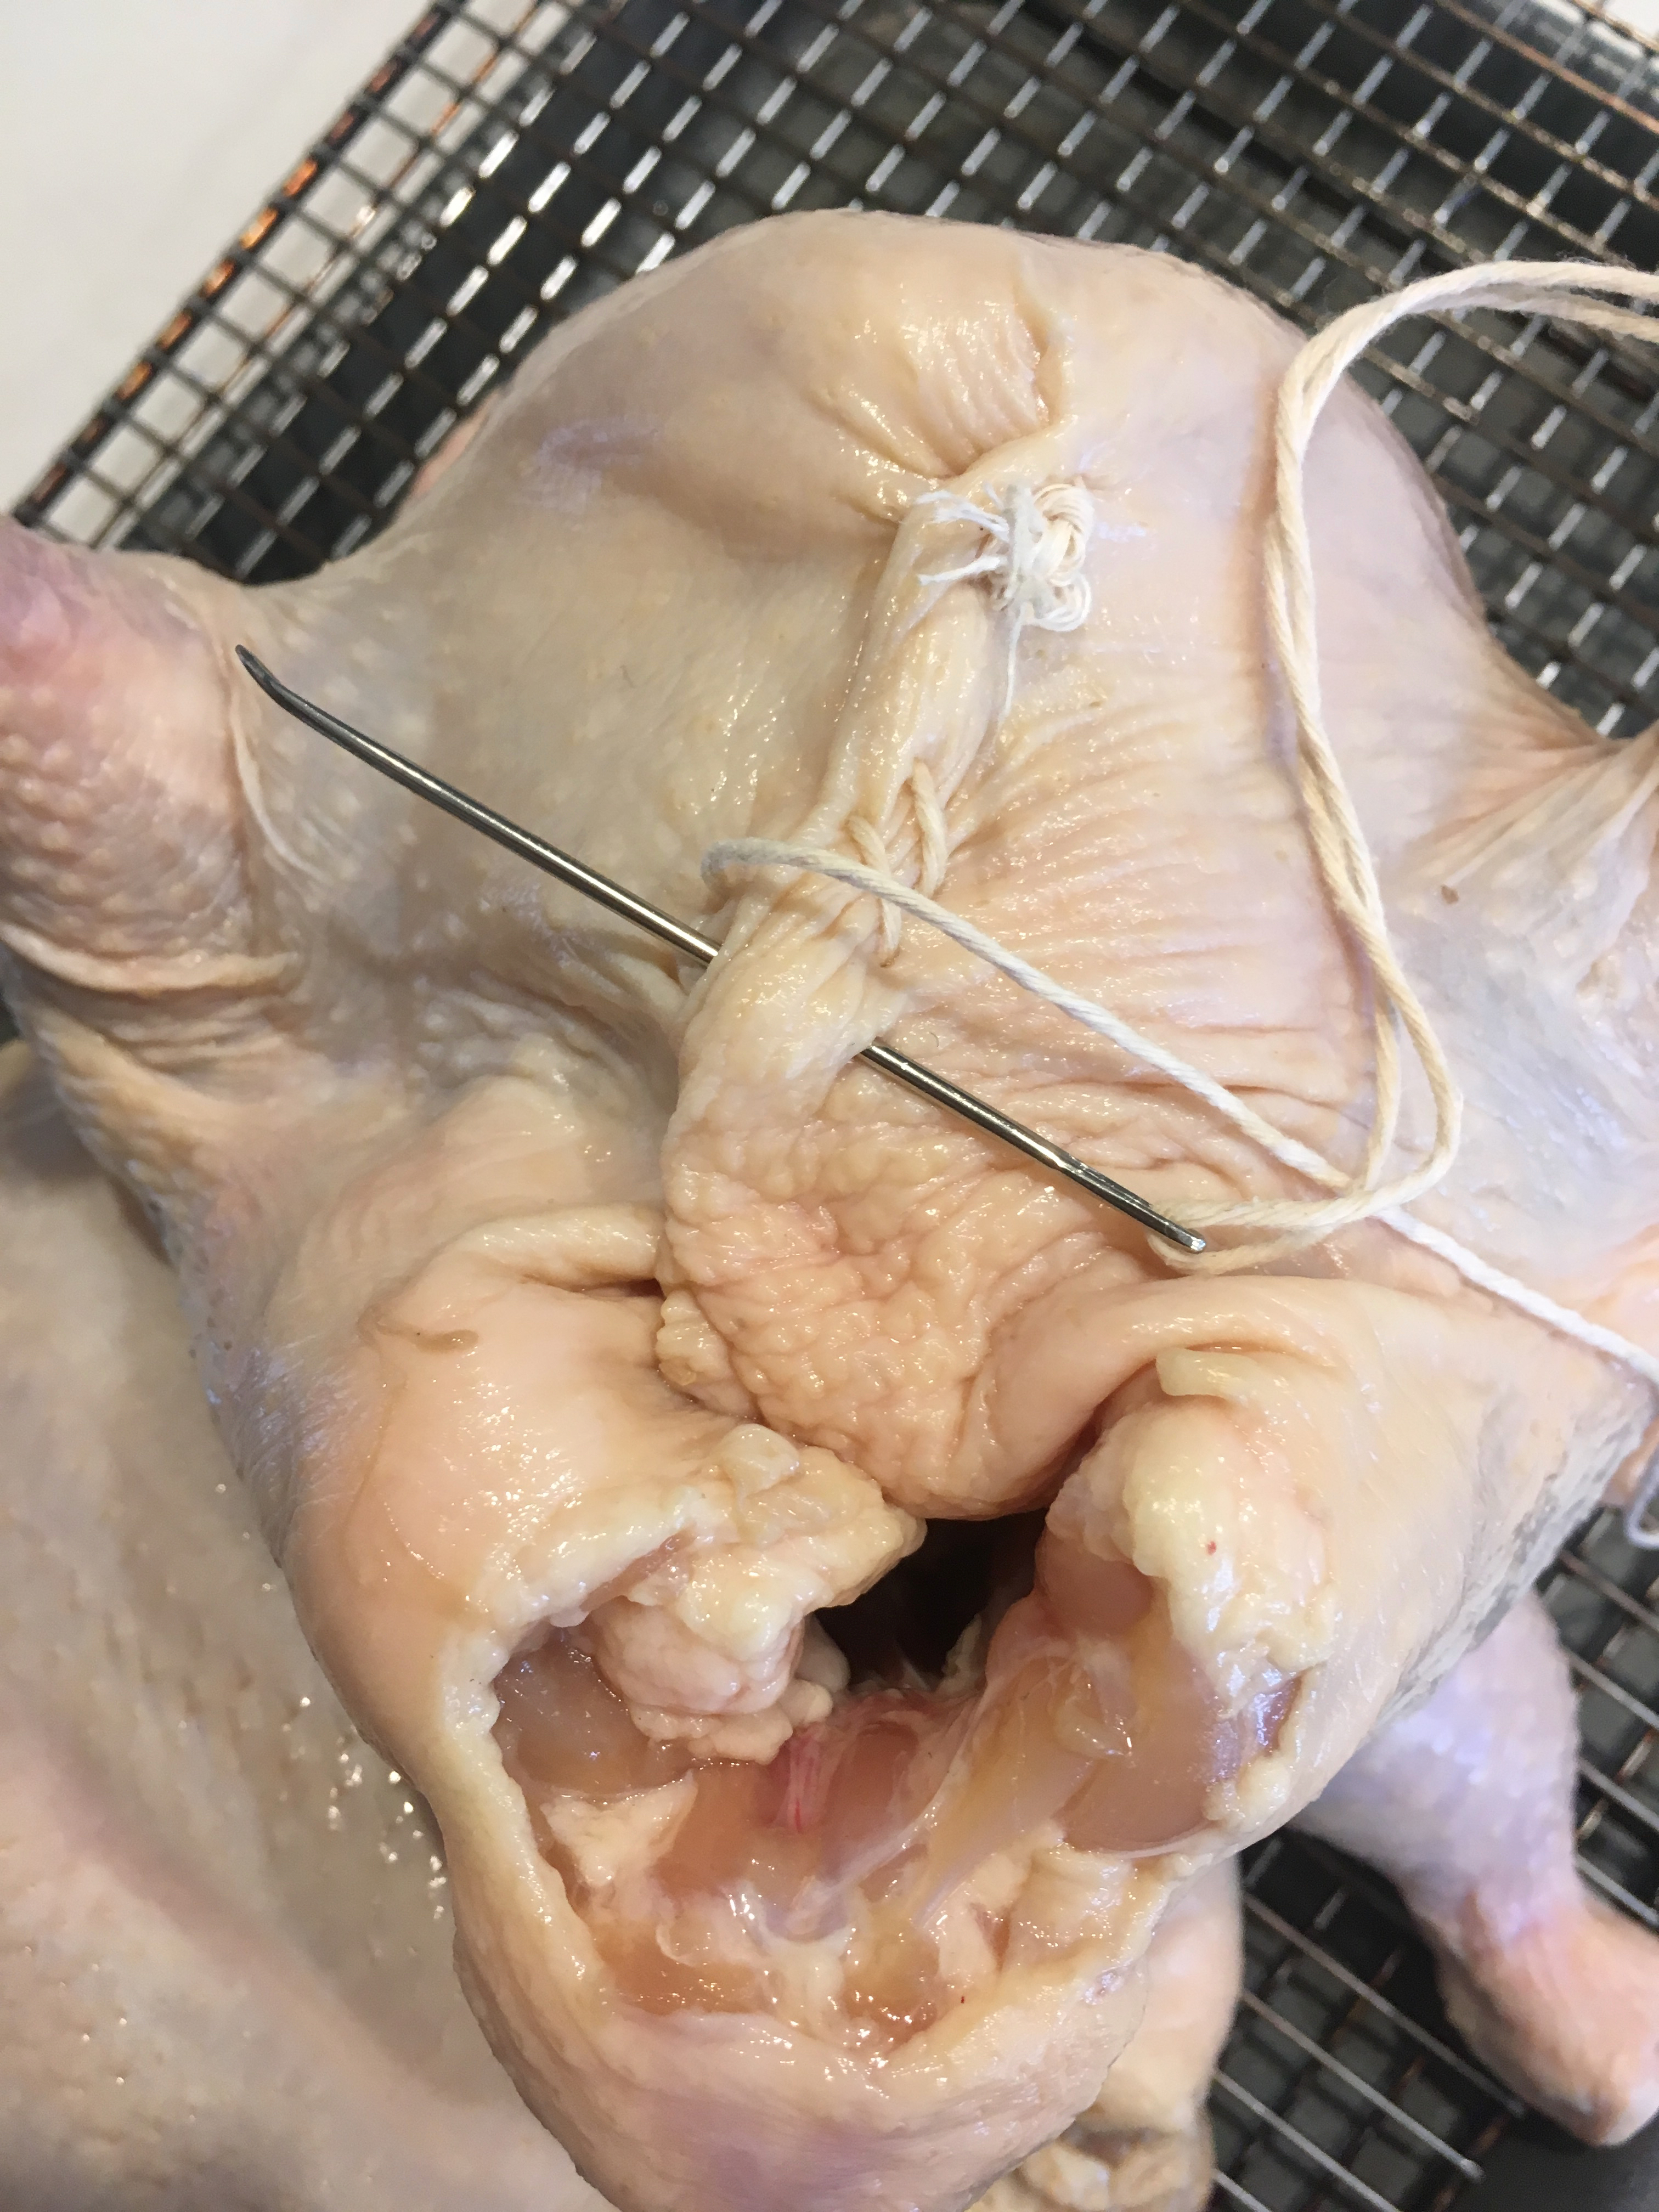
\includegraphics[width=0.25\textwidth]{\imageDir/\fileName/IMG_3214.jpg} &
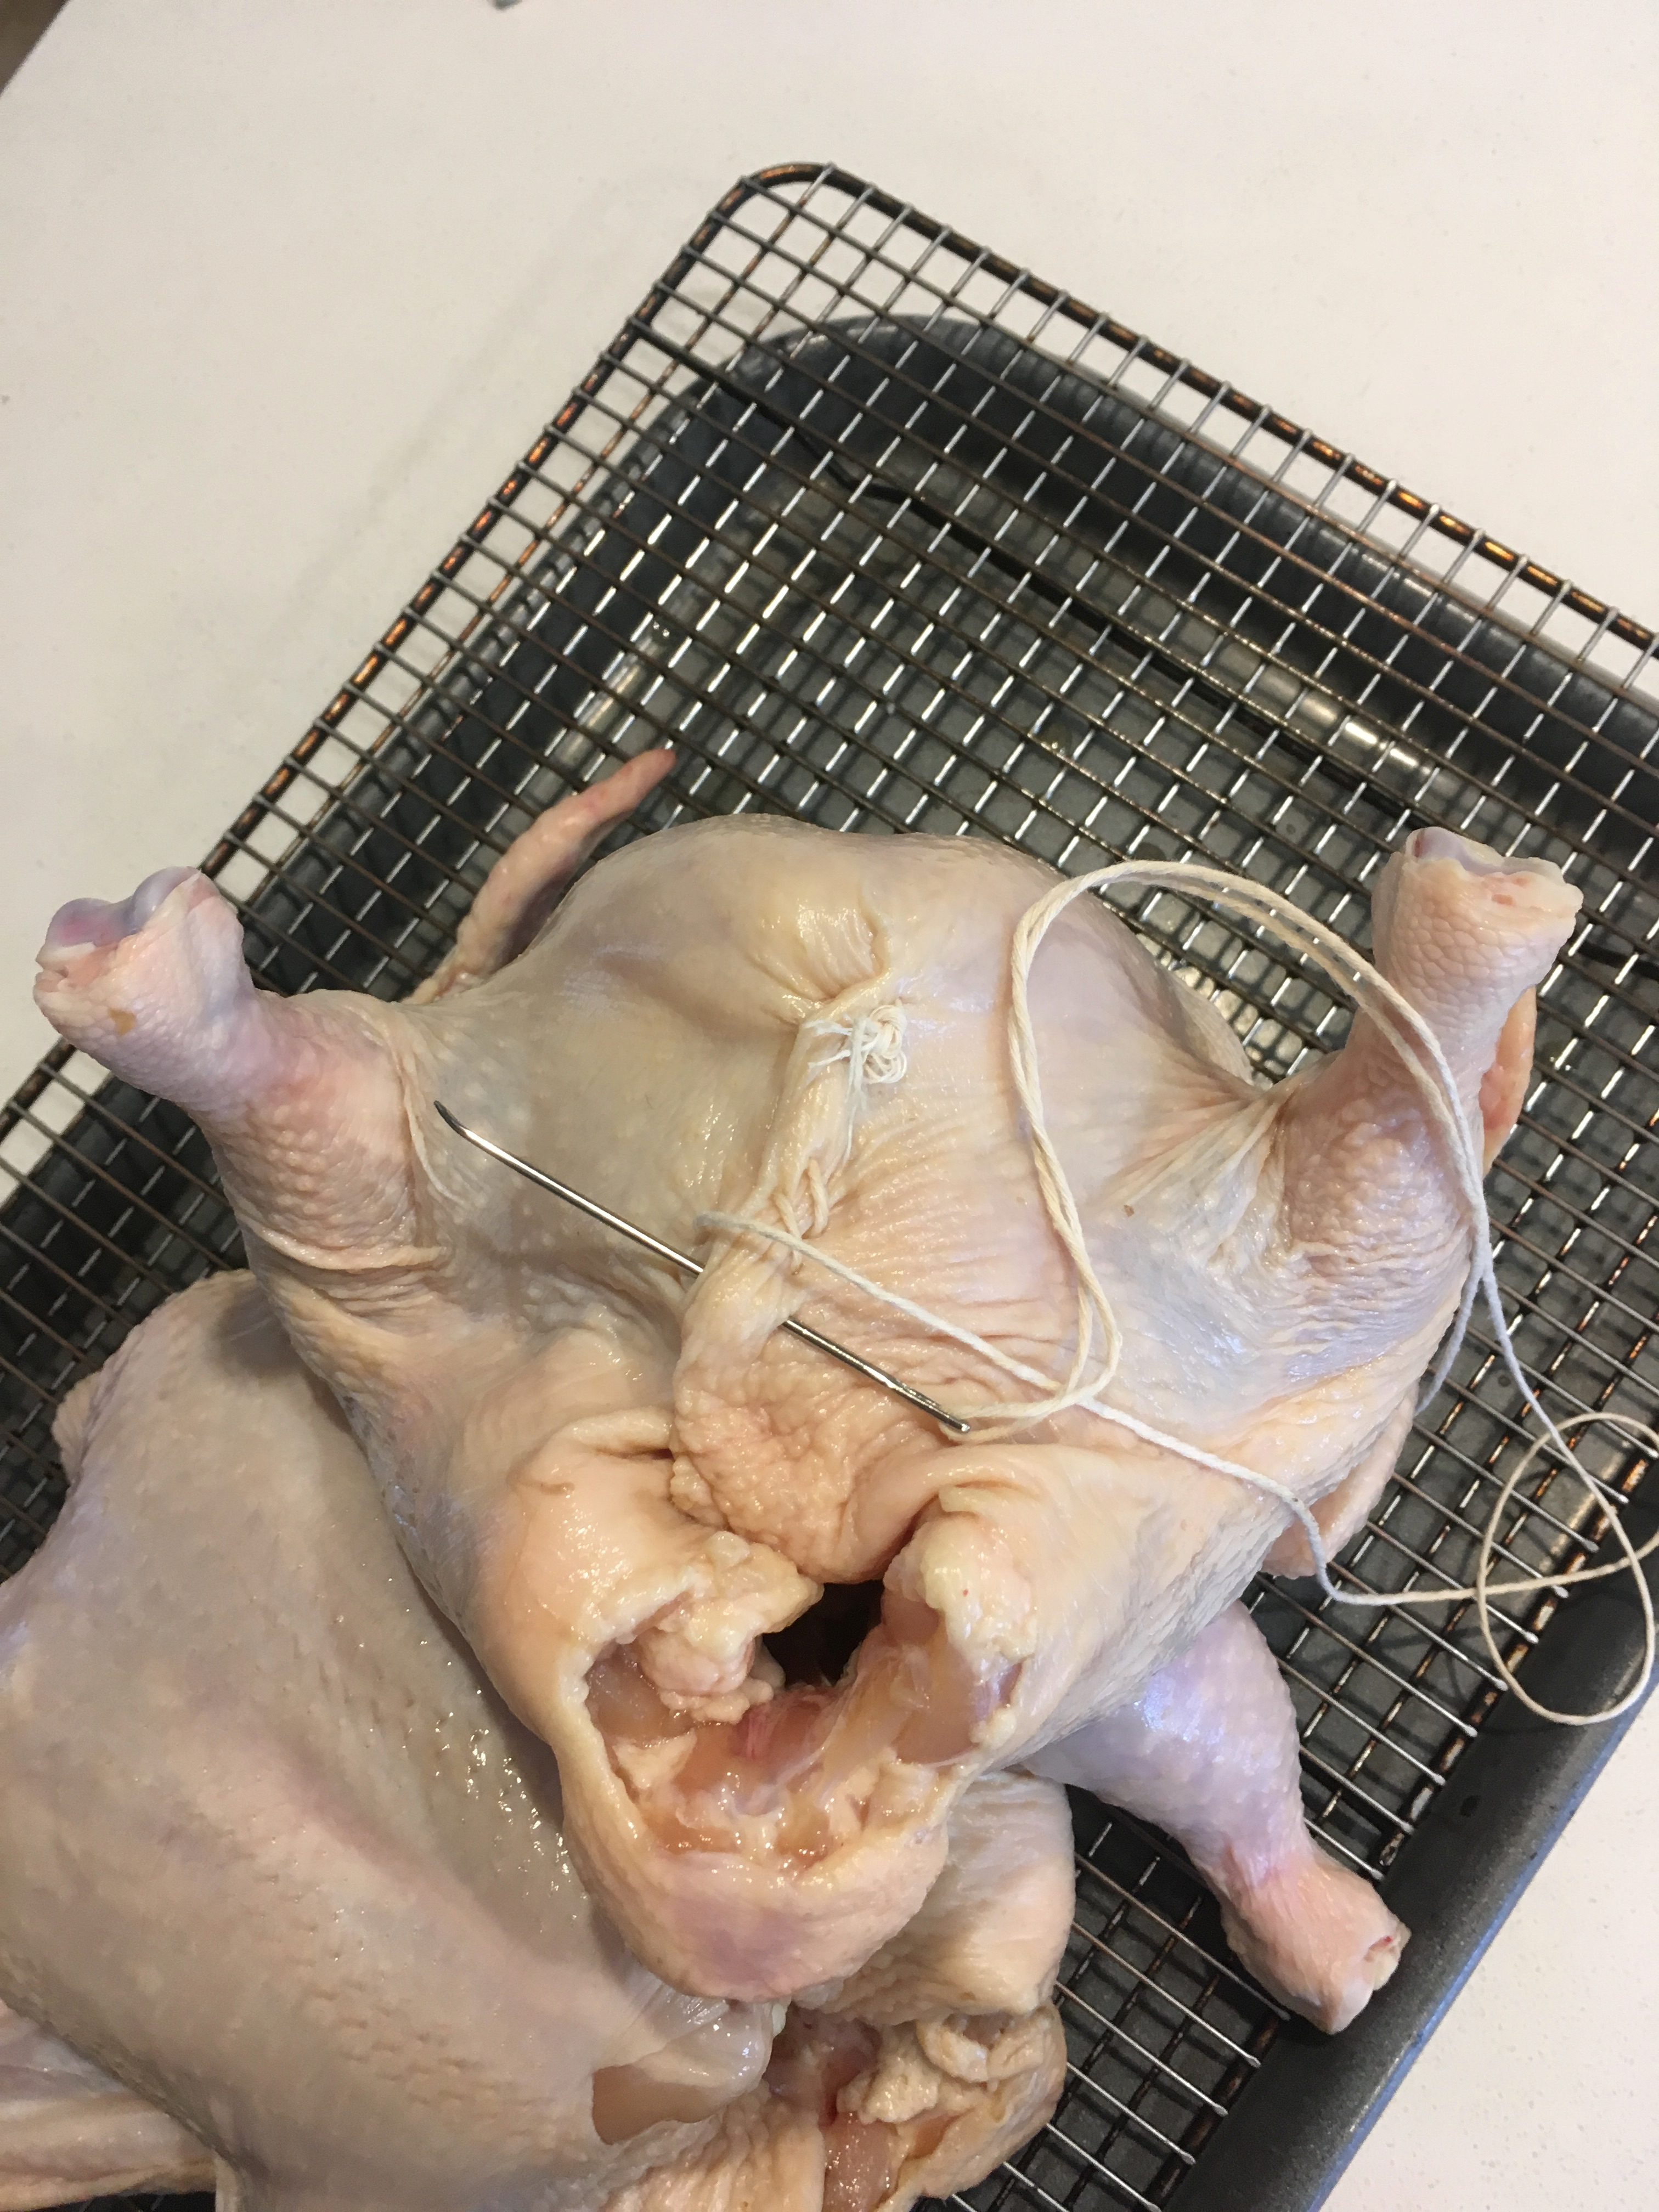
\includegraphics[width=0.25\textwidth]{\imageDir/\fileName/IMG_3216.jpg} \\
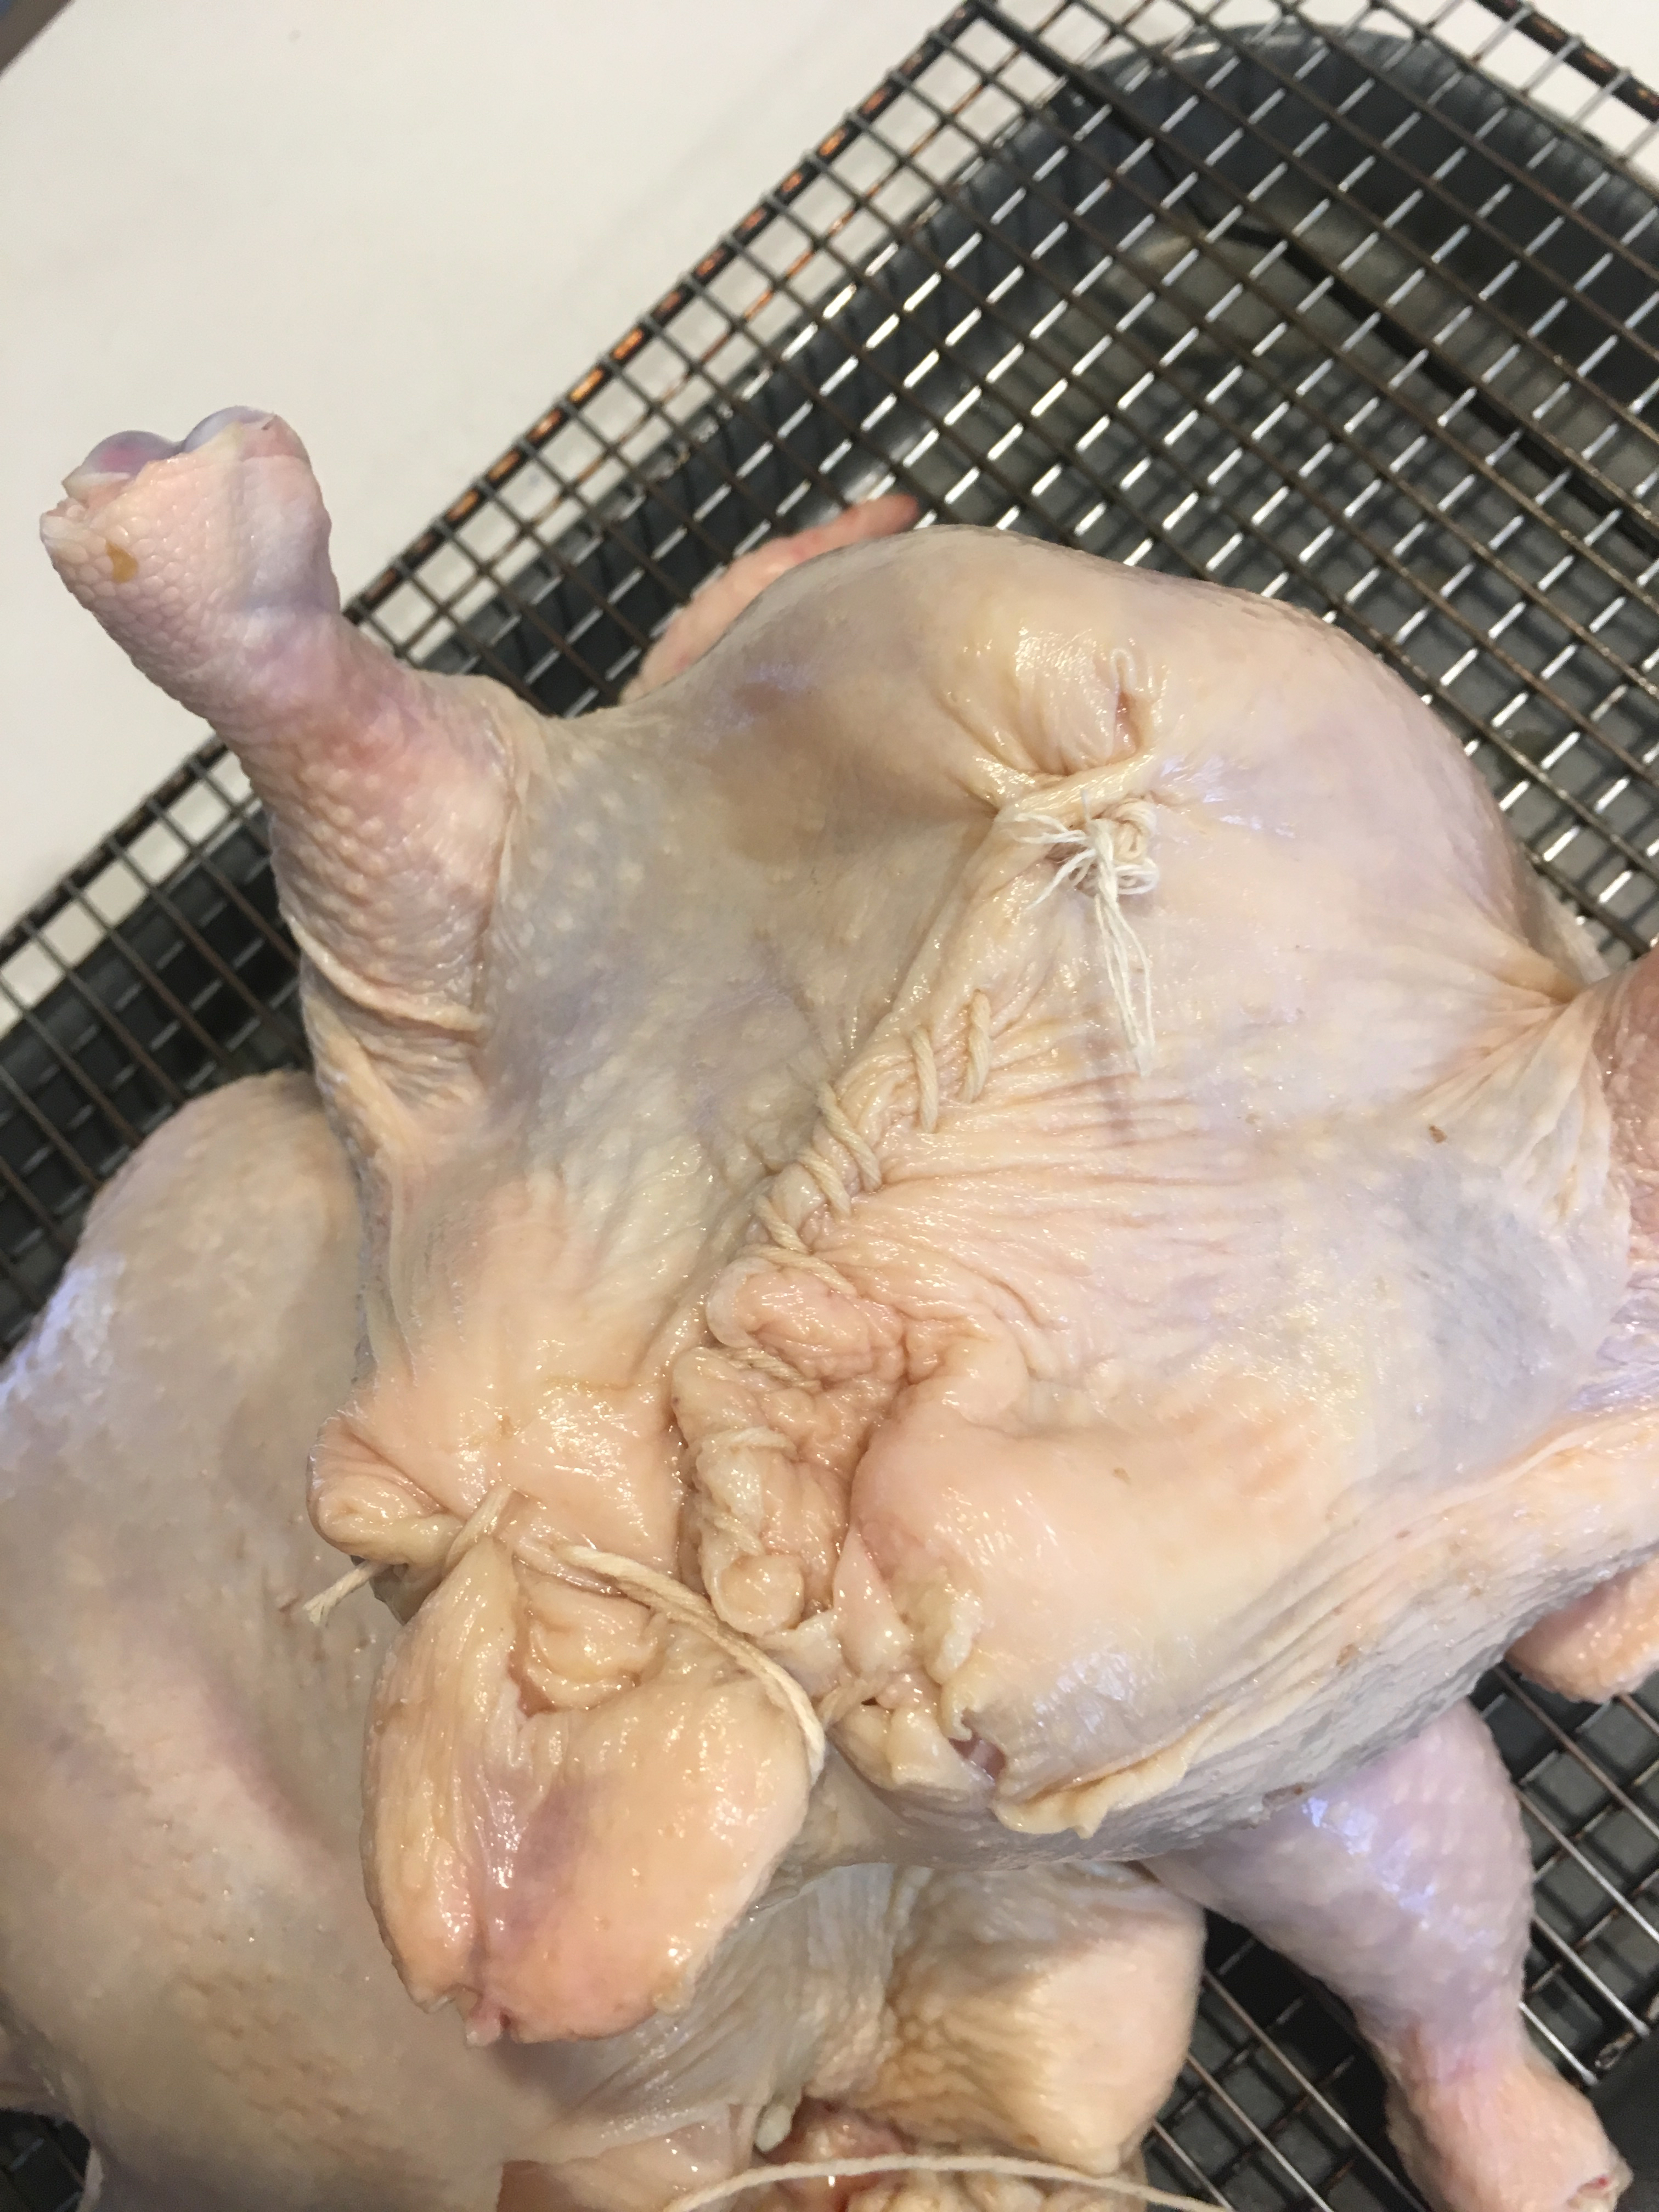
\includegraphics[width=0.25\textwidth]{\imageDir/\fileName/IMG_3217.jpg} &
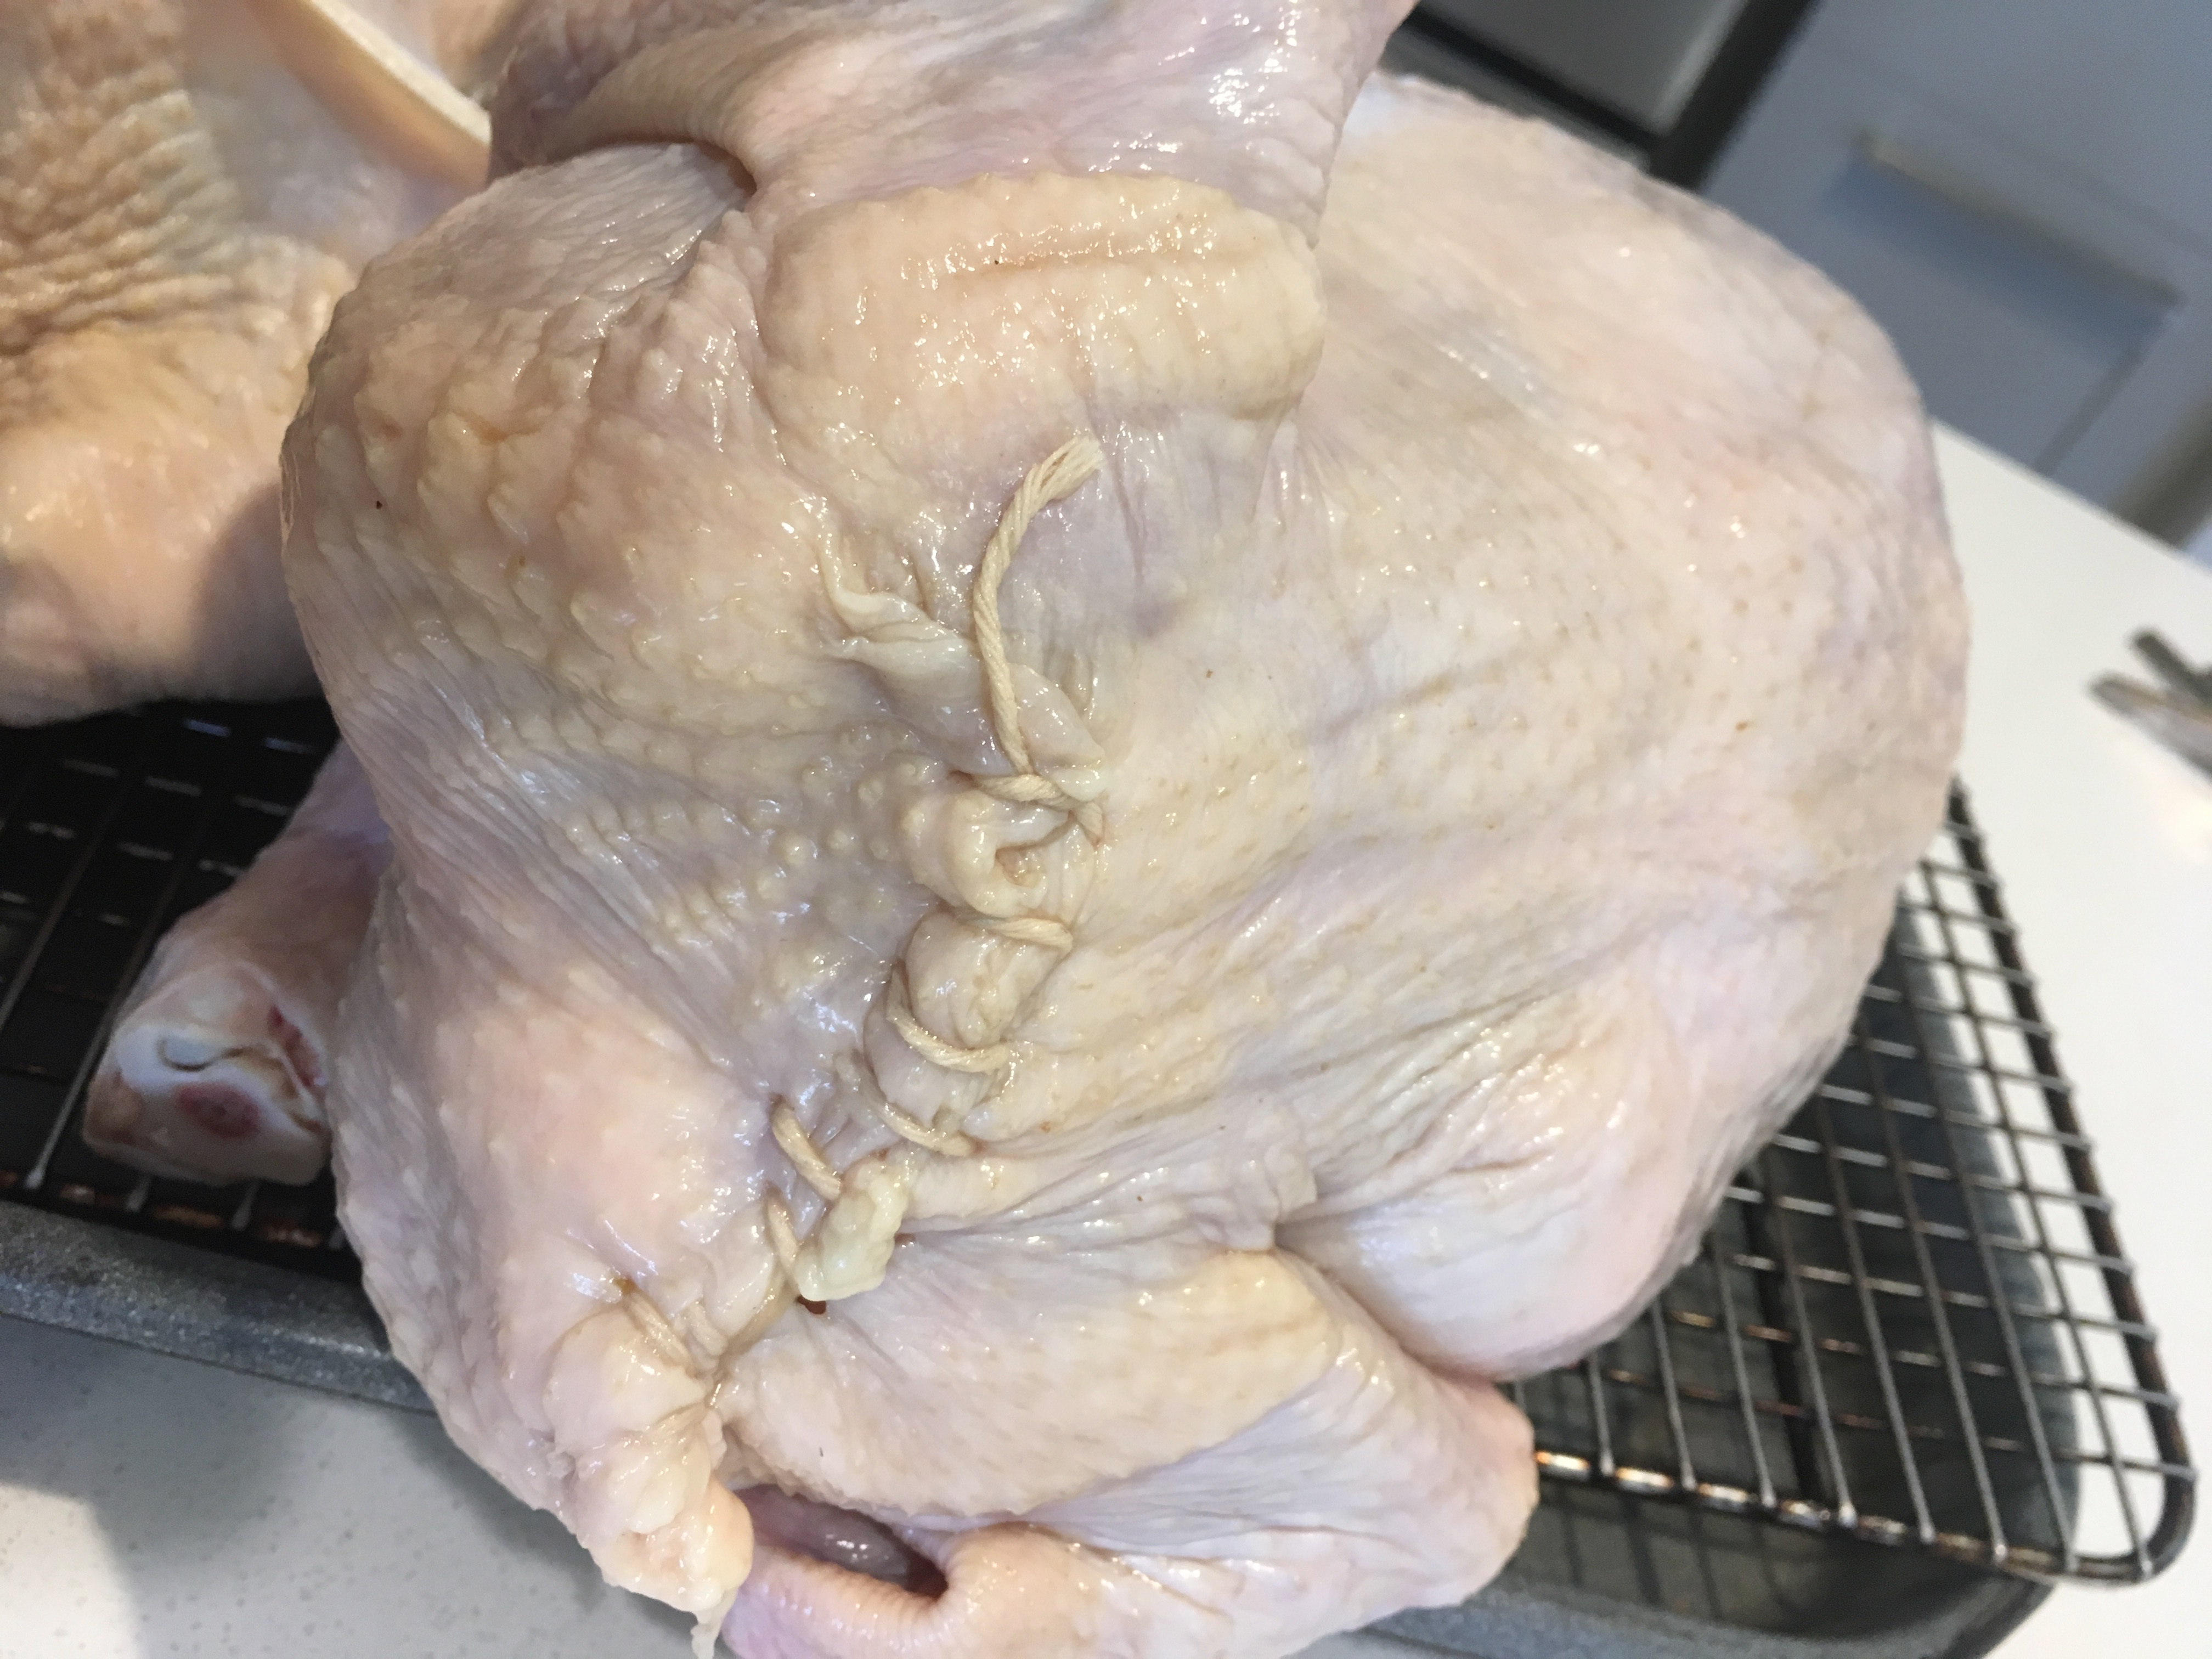
\includegraphics[width=0.25\textwidth]{\imageDir/\fileName/IMG_3218.jpg} &
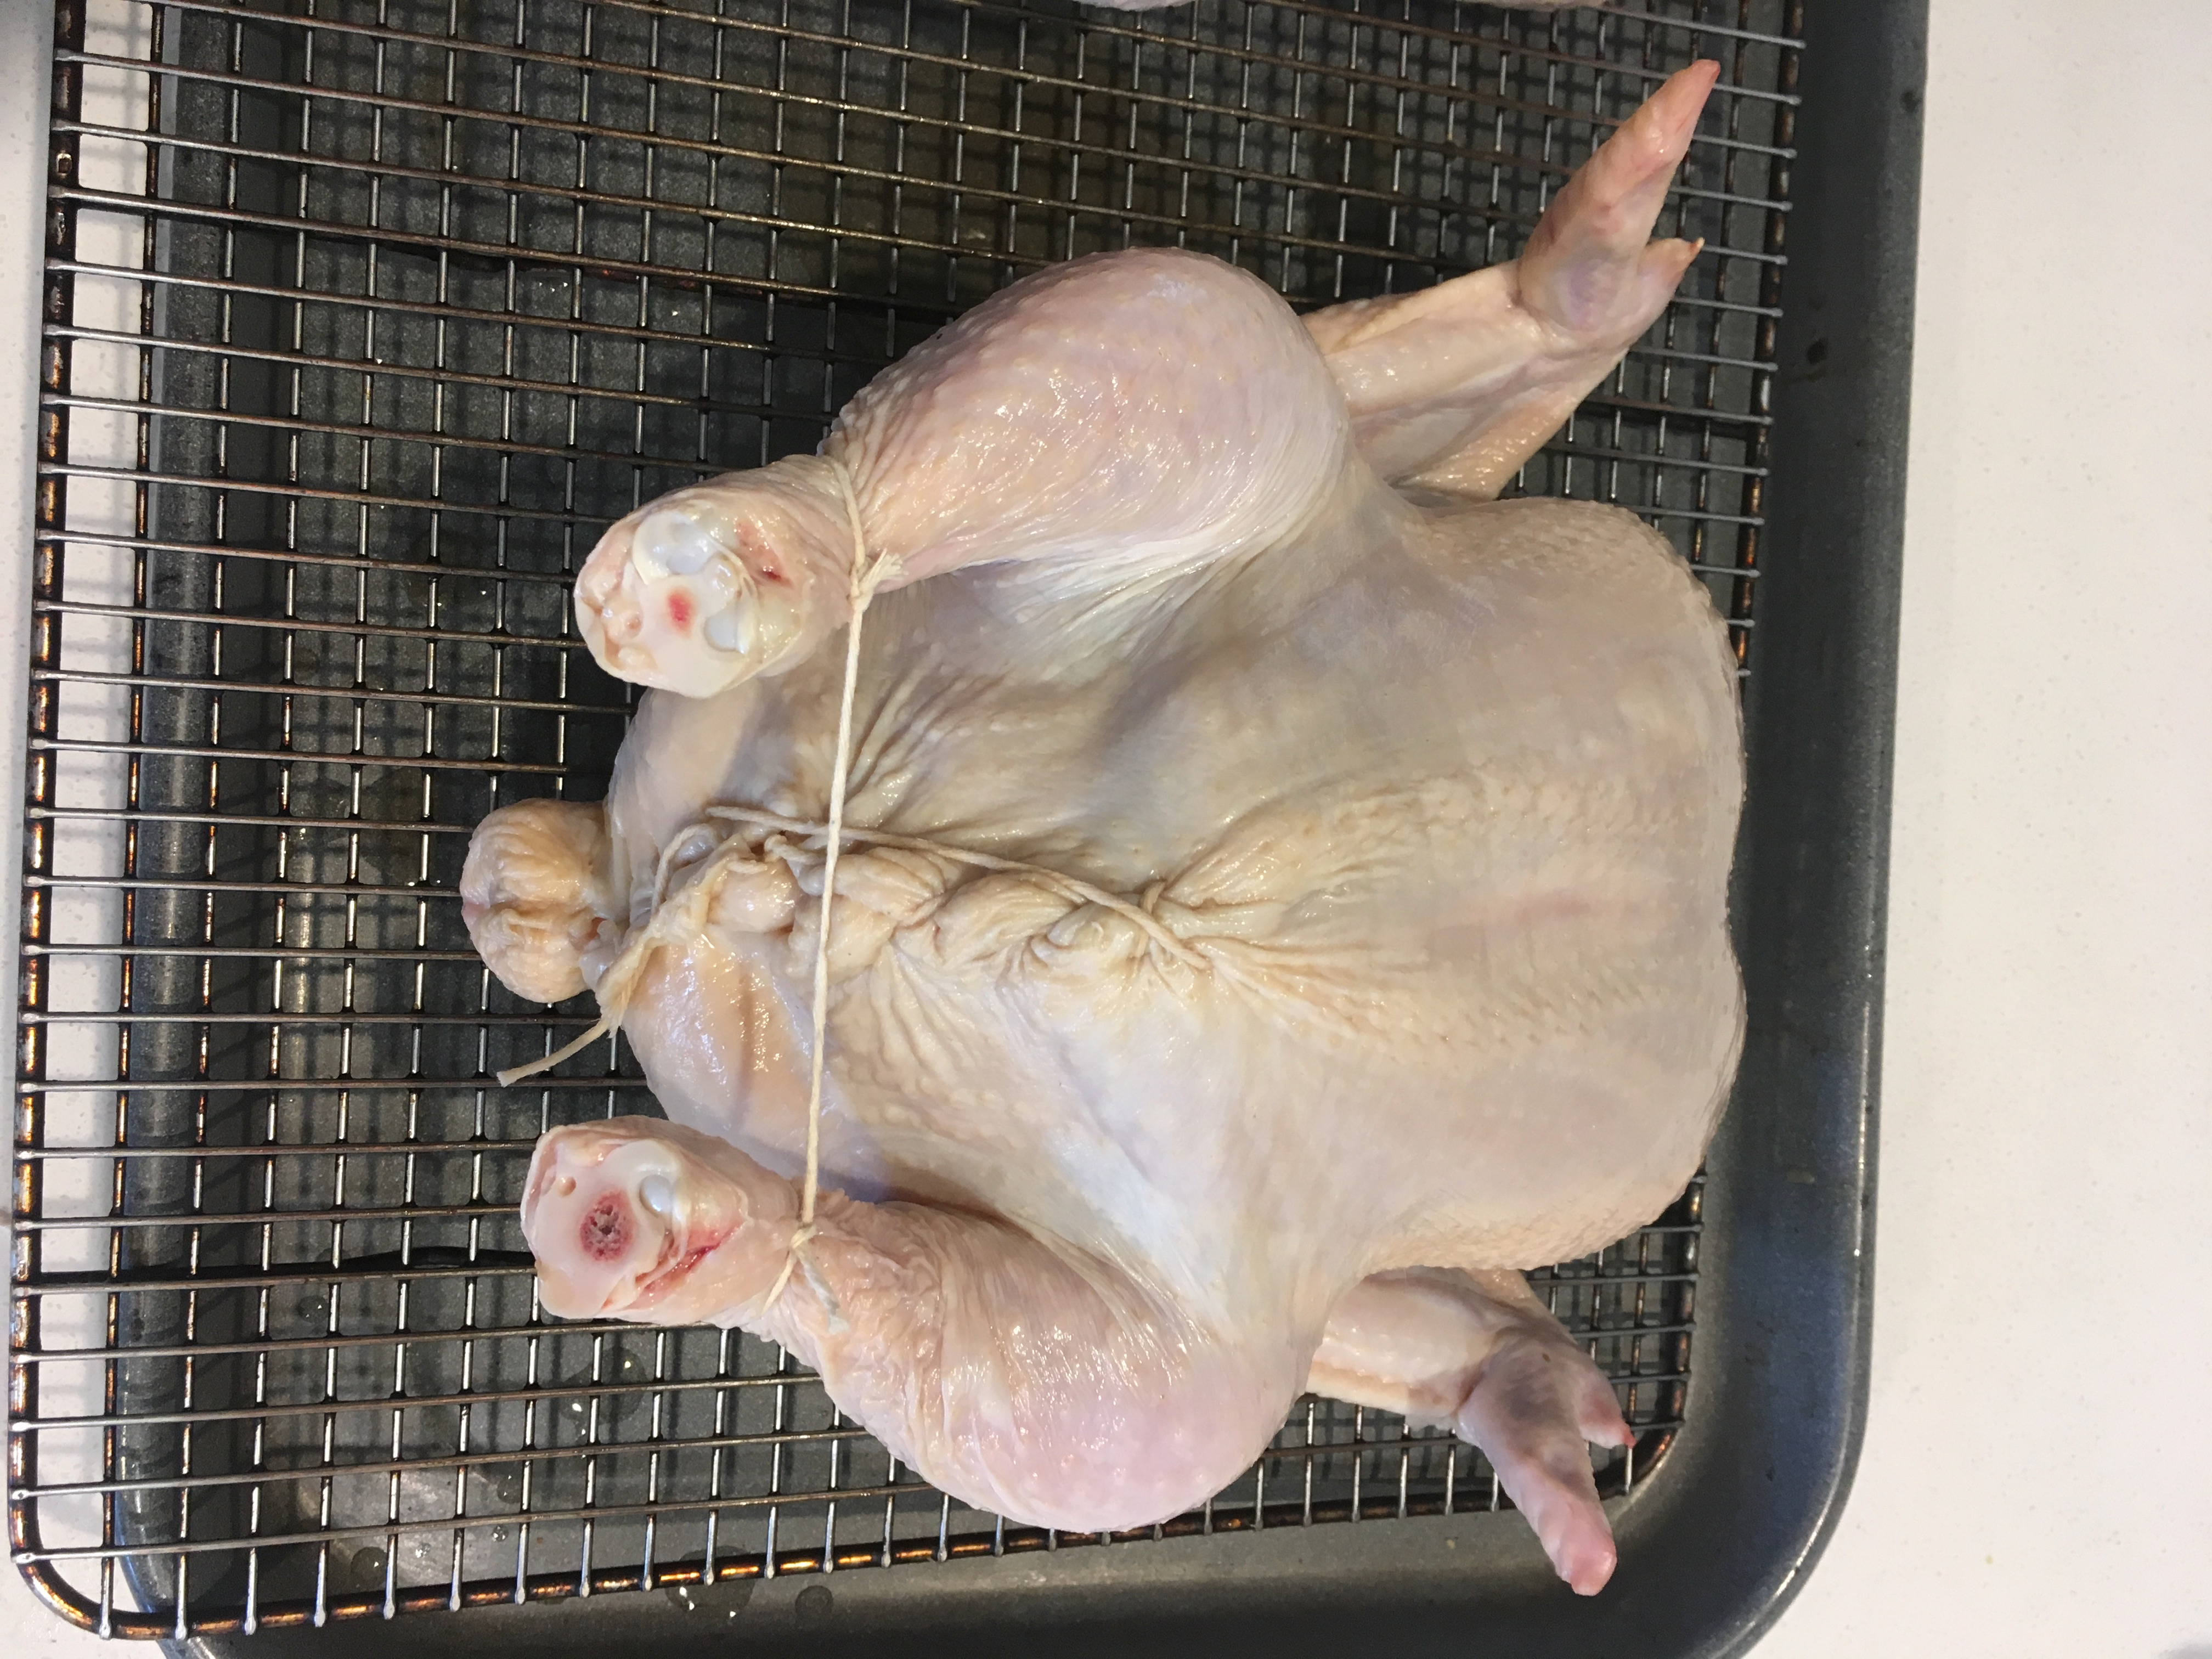
\includegraphics[width=0.25\textwidth]{\imageDir/\fileName/IMG_3219.jpg} \\
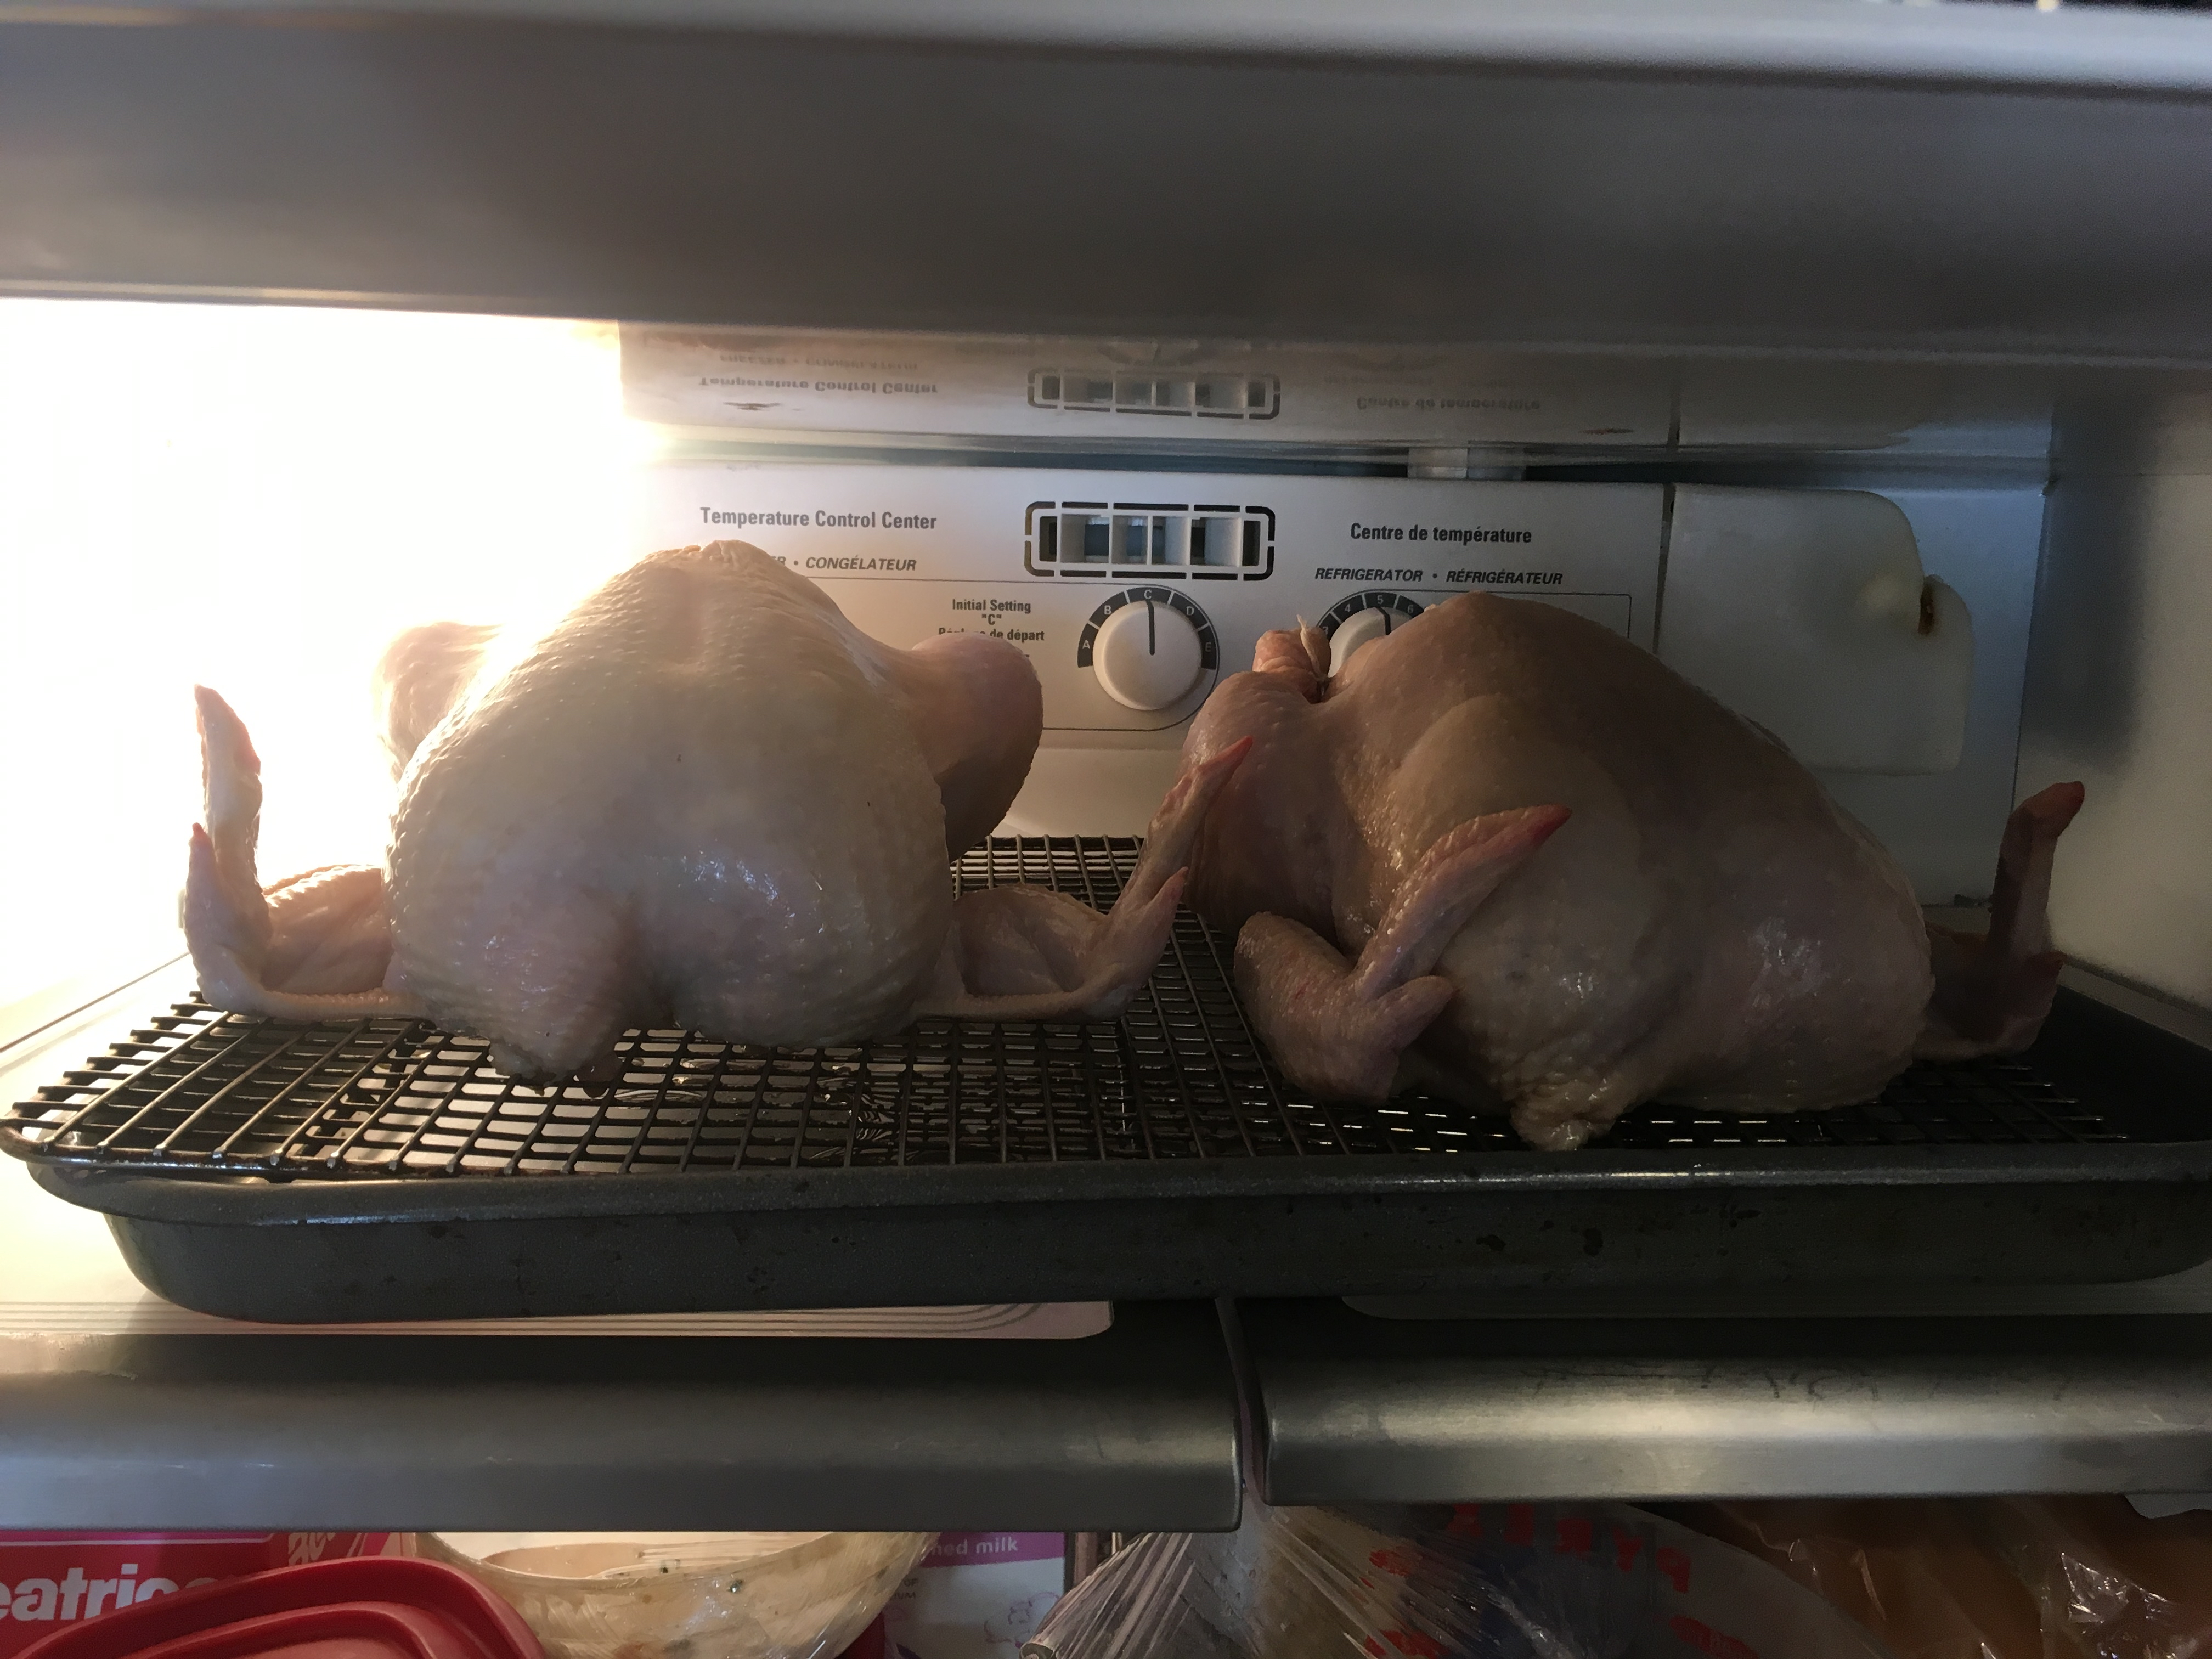
\includegraphics[width=0.25\textwidth]{\imageDir/\fileName/IMG_3220.jpg} &
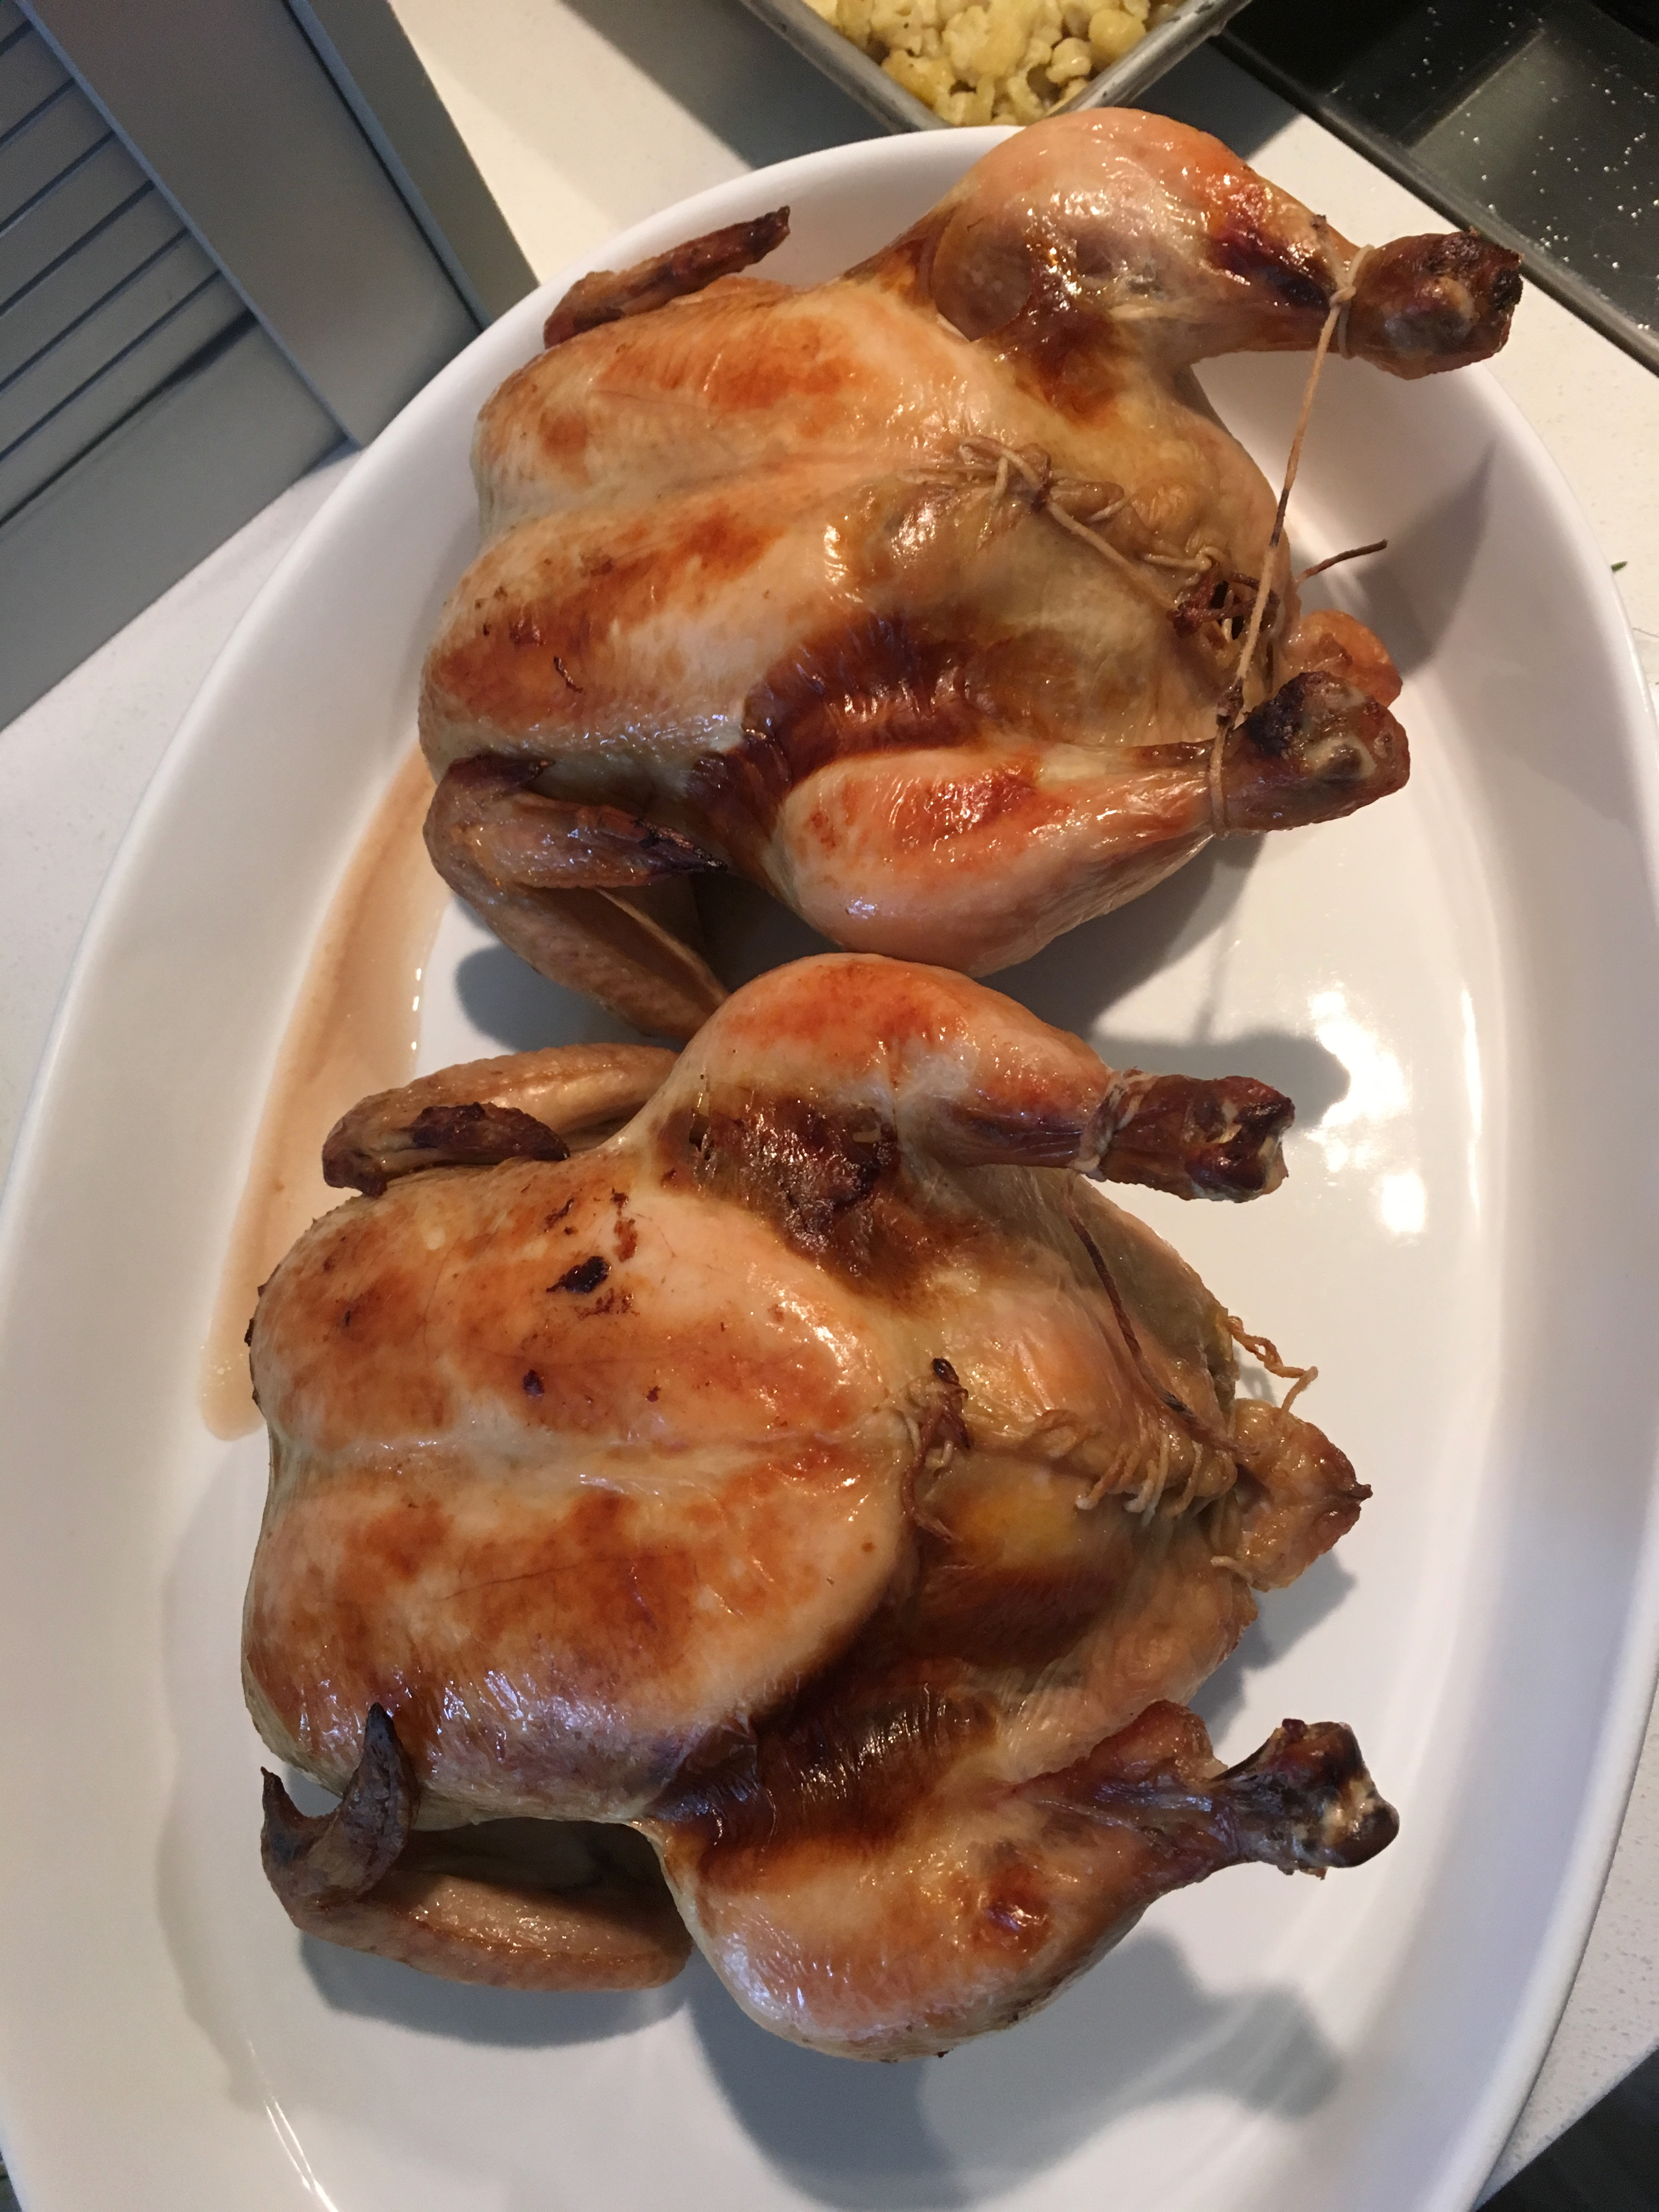
\includegraphics[width=0.25\textwidth]{\imageDir/\fileName/IMG_3228.jpg} \\
\end{tabular}
\end{table}

\end{document}



